% !TeX spellcheck = pl_PL
%%%%%%%%%%%%%%%%%%%%%%%%%%%%%%%%%%%%%%%%%%%
%                                        %
% Szablon pracy dyplomowej inzynierskiej %
% zgodny  z aktualnymi  przepisami  SZJK %
%                                        %
%%%%%%%%%%%%%%%%%%%%%%%%%%%%%%%%%%%%%%%%%%
%                                        %
%  (c) Krzysztof Simiński, 2018-2023     %
%                                        %
%%%%%%%%%%%%%%%%%%%%%%%%%%%%%%%%%%%%%%%%%%
%                                        %
% Najnowsza wersja szablonów jest        %
% podstępna pod adresem                  %
% github.com/ksiminski/polsl-aei-theses  %
%                                        %
%%%%%%%%%%%%%%%%%%%%%%%%%%%%%%%%%%%%%%%%%%
%
%
% Projekt LaTeXowy zapewnia odpowiednie formatowanie pracy,
% zgodnie z wymaganiami Systemu zapewniania jakości kształcenia.
% Proszę nie zmieniać ustawień formatowania (np. fontu,
% marginesów, wytłuszczeń, kursywy itd. ).
%
% Projekt można kompilować na kilka sposobów.
%
% 1. kompilacja pdfLaTeX
%
% pdflatex main
% bibtex   main
% pdflatex main
% pdflatex main
%
%
% 2. kompilacja XeLaTeX
%
% Kompilatacja przy użyciu XeLaTeXa różni się tym, że na stronie
% tytułowej używany jest font Calibri. Wymaga to jego uprzedniego
% zainstalowania.
%
% xelatex main
% bibtex  main
% xelatex main
% xelatex main
%
%
%%%%%%%%%%%%%%%%%%%%%%%%%%%%%%%%%%%%%%%%%%%%%%%%%%%%%
% W przypadku pytań, uwag, proszę pisać na adres:   %
%      krzysztof.siminski(małpa)polsl.pl            %
%%%%%%%%%%%%%%%%%%%%%%%%%%%%%%%%%%%%%%%%%%%%%%%%%%%%%
%
% Chcemy ulepszać szablony LaTeXowe prac dyplomowych.
% Wypełniając ankietę spod poniższego adresu pomogą
% Państwo nam to zrobić. Ankieta jest całkowicie
% anonimowa. Dziękujemy!


% https://docs.google.com/forms/d/e/1FAIpQLScyllVxNKzKFHfILDfdbwC-jvT8YL0RSTFs-s27UGw9CKn-fQ/viewform?usp=sf_link
%
%%%%%%%%%%%%%%%%%%%%%%%%%%%%%%%%%%%%%%%%%%%%%%%%%%%%%%%%%%%%%%%%%%%%%%%%%

%%%%%%%%%%%%%%%%%%%%%%%%%%%%%%%%%%%%%%%%%%%%%%%
%                                             %
% PERSONALIZACJA PRACY – DANE PRACY           %
%                                             %
%%%%%%%%%%%%%%%%%%%%%%%%%%%%%%%%%%%%%%%%%%%%%%%

% Proszę wpisać swoje dane w poniższych definicjach.

% TODO
% dane autora
\newcommand{\FirstNameAuthor}{Jakub}
\newcommand{\SurnameAuthor}{Kula}
\newcommand{\IdAuthor}{296849}   % numer albumu  (bez $\langle$ i $\rangle$)

% drugi autor:
%\newcommand{\FirstNameCoauthor}{Imię}   % Jeżeli jest drugi autor, to tutaj należy podać imię.
%\newcommand{\SurnameCoauthor}{Nazwisko} % Jeżeli jest drugi autor, to tutaj należy podać nazwisko.
%\newcommand{\IdCoauthor}{$\langle$wpisać właściwy$\rangle$}  % numer albumu drugiego autora (bez $\langle$ i $\rangle$)
% Gdy nie ma drugiego autora, należy zostawić poniższe definicje puste, jak poniżej. Gdy jest drugi autor, należy zakomentować te linie.
\newcommand{\FirstNameCoauthor}{} % Jeżeli praca ma tylko jednego autora, to dane drugiego autora zostają puste.
\newcommand{\SurnameCoauthor}{}   % Jeżeli praca ma tylko jednego autora, to dane drugiego autora zostają puste.
\newcommand{\IdCoauthor}{}  % Jeżeli praca ma tylko jednego autora, to dane drugiego autora zostają puste.
%%%%%%%%%%

\newcommand{\Supervisor}{dr inż. Szymon Ogonowski, prof. PŚ}     % dane promotora (bez $\langle$ i $\rangle$)
\newcommand{\Title}{Modelowanie i analiza procesów związanych z działaniem systemu centralnego ogrzewania oraz przygotowania wody użytkowej w budynku mieszkalnym z wykorzystaniem uczenia maszynowego}           % tytuł pracy po polsku
\newcommand{\TitleAlt}{Modeling and analysis of the heating and hot water preparation processes in residential building using machine learning}                     % thesis title in English
\newcommand{\Program}{Automatyka i Robotyka}            % kierunek studiów  (bez $\langle$ i $\rangle$)
\newcommand{\Specialisation}{Technologie Informacyjne}     % specjalność  (bez $\langle$ i $\rangle$)
\newcommand{\Departament}{Katedry Pomiarów i Systemów Sterowania}        % katedra promotora  (bez $\langle$ i $\rangle$)

% Jeżeli został wyznaczony promotor pomocniczy lub opiekun, proszę go/ją wpisać ...
\newcommand{\Consultant}{} % dane promotora pomocniczego, opiekuna (bez $\langle$ i $\rangle$)
% ... w przeciwnym razie proszę zostawić puste miejsce jak poniżej:
%\newcommand{\Consultant}{} % brak promotowa pomocniczego / opiekuna

% koniec fragmentu do modyfikacji
%%%%%%%%%%%%%%%%%%%%%%%%%%%%%%%%%%%%%%%%%%


%%%%%%%%%%%%%%%%%%%%%%%%%%%%%%%%%%%%%%%%%%%%%%%
%                                             %
% KONIEC PERSONALIZACJI PRACY                 %
%                                             %
%%%%%%%%%%%%%%%%%%%%%%%%%%%%%%%%%%%%%%%%%%%%%%%

%%%%%%%%%%%%%%%%%%%%%%%%%%%%%%%%%%%%%%%%


%%%%%%%%%%%%%%%%%%%%%%%%%%%%%%%%%%%%%%%%%%%%%%%
%                                             %
% PROSZĘ NIE MODYFIKOWAĆ PONIŻSZYCH USTAWIEŃ! %
%                                             %
%%%%%%%%%%%%%%%%%%%%%%%%%%%%%%%%%%%%%%%%%%%%%%%



\documentclass[a4paper,twoside,12pt]{book}
\usepackage[utf8]{inputenc}                                      
\usepackage[T1]{fontenc}  
\usepackage{amsmath,amsfonts,amssymb,amsthm}
\usepackage[british,polish]{babel} 
\usepackage{indentfirst}
\usepackage{xurl}
\usepackage{xstring}
\usepackage{ifthen}

\usepackage{multirow}


\usepackage{ifxetex}

\ifxetex
	\usepackage{fontspec}
	\defaultfontfeatures{Mapping=tex—text} % to support TeX conventions like ``——-''
	\usepackage{xunicode} % Unicode support for LaTeX character names (accents, European chars, etc)
	\usepackage{xltxtra} % Extra customizations for XeLaTeX
\else
	\usepackage{lmodern}
\fi



\usepackage[margin=2.5cm]{geometry}
\usepackage{graphicx} 
\usepackage{hyperref}
\usepackage{booktabs}
\usepackage{tikz}
\usepackage{ circuitikz }
\usepackage{pgfplots}
\usepackage{mathtools}
\usepackage{geometry}
\usepackage{subcaption}   % subfigures
\usepackage[page]{appendix} % toc,
\renewcommand{\appendixtocname}{Dodatki}
\renewcommand{\appendixpagename}{Dodatki}
\renewcommand{\appendixname}{Dodatek}

\usepackage{csquotes}
\usepackage[natbib=true,backend=bibtex,maxbibnames=99]{biblatex}  % kompilacja bibliografii BibTeXem
%\usepackage[natbib=true,backend=biber,maxbibnames=99]{biblatex}  % kompilacja bibliografii Biberem
\bibliography{biblio}

\usepackage{ifmtarg}   % empty commands  

\usepackage{setspace}
\onehalfspacing


\frenchspacing



%%%% TODO LIST GENERATOR %%%%%%%%%

\usepackage{color}
\definecolor{brickred}      {cmyk}{0   , 0.89, 0.94, 0.28}

\makeatletter \newcommand \kslistofremarks{\section*{Uwagi} \@starttoc{rks}}
  \newcommand\l@uwagas[2]
    {\par\noindent \textbf{#2:} %\parbox{10cm}
{#1}\par} \makeatother


\newcommand{\ksremark}[1]{%
{%\marginpar{\textdbend}
{\color{brickred}{[#1]}}}%
\addcontentsline{rks}{uwagas}{\protect{#1}}%
}

\newcommand{\comma}{\ksremark{przecinek}}
\newcommand{\nocomma}{\ksremark{bez przecinka}}
\newcommand{\styl}{\ksremark{styl}}
\newcommand{\ortografia}{\ksremark{ortografia}}
\newcommand{\fleksja}{\ksremark{fleksja}}
\newcommand{\pauza}{\ksremark{pauza `--', nie dywiz `-'}}
\newcommand{\kolokwializm}{\ksremark{kolokwializm}}
\newcommand{\cudzyslowy}{\ksremark{,,polskie cudzysłowy''}}

%%%%%%%%%%%%%% END OF TODO LIST GENERATOR %%%%%%%%%%%

\newcommand{\printCoauthor}{%		
    \StrLen{\FirstNameCoauthor}[\FNCoALen]
    \ifthenelse{\FNCoALen > 0}%
    {%
		{\large\bfseries\Coauthor\par}
	
		{\normalsize\bfseries \LeftId: \IdCoauthor\par}
    }%
    {}
} 

%%%%%%%%%%%%%%%%%%%%%
\newcommand{\autor}{%		
    \StrLen{\FirstNameCoauthor}[\FNCoALenXX]
    \ifthenelse{\FNCoALenXX > 0}%
    {\FirstNameAuthor\ \SurnameAuthor, \FirstNameCoauthor\ \SurnameCoauthor}%
	{\FirstNameAuthor\ \SurnameAuthor}%
}
%%%%%%%%%%%%%%%%%%%%%

\StrLen{\FirstNameCoauthor}[\FNCoALen]
\ifthenelse{\FNCoALen > 0}%
{%
\author{\FirstNameAuthor\ \SurnameAuthor, \FirstNameCoauthor\ \SurnameCoauthor}
}%
{%
\author{\FirstNameAuthor\ \SurnameAuthor}
}%

%%%%%%%%%%%% ZYWA PAGINA %%%%%%%%%%%%%%%
% brak kapitalizacji zywej paginy
\usepackage{fancyhdr}
\pagestyle{fancy}
\fancyhf{}
\fancyhead[LO]{\nouppercase{\it\rightmark}}
\fancyhead[RE]{\nouppercase{\it\leftmark}}
\fancyhead[LE,RO]{\it\thepage}


\fancypagestyle{tylkoNumeryStron}{%
   \fancyhf{} 
   \fancyhead[LE,RO]{\it\thepage}
}

\fancypagestyle{bezNumeracji}{%
   \fancyhf{} 
   \fancyhead[LE,RO]{}
}


\fancypagestyle{NumeryStronNazwyRozdzialow}{%
   \fancyhf{} 
   \fancyhead[LE]{\nouppercase{\autor}}
   \fancyhead[RO]{\nouppercase{\leftmark}} 
   \fancyfoot[CE, CO]{\thepage}
}


%%%%%%%%%%%%% OBCE WTRETY  
\newcommand{\obcy}[1]{\emph{#1}}
\newcommand{\english}[1]{{\selectlanguage{british}\obcy{#1}}}
%%%%%%%%%%%%%%%%%%%%%%%%%%%%%

% polskie oznaczenia funkcji matematycznych
\renewcommand{\tan}{\operatorname {tg}}
\renewcommand{\log}{\operatorname {lg}}

% jeszcze jakies drobiazgi

\newcounter{stronyPozaNumeracja}

%%%%%%%%%%%%%%%%%%%%%%%%%%% 
\newcommand{\printOpiekun}[1]{%		

    \StrLen{\Consultant}[\mystringlen]
    \ifthenelse{\mystringlen > 0}%
    {%
       {\large{\bfseries OPIEKUN, PROMOTOR POMOCNICZY}\par}
       
       {\large{\bfseries \Consultant}\par}
    }%
    {}
} 
%
%%%%%%%%%%%%%%%%%%%%%%%%%%%%%%%%%%%%%%%%%%%%%%
 
% Proszę nie modyfikować poniższych definicji!
\newcommand{\Author}{\FirstNameAuthor\ \MakeUppercase{\SurnameAuthor}} 
\newcommand{\Coauthor}{\FirstNameCoauthor\ \MakeUppercase{\SurnameCoauthor}}
\newcommand{\Type}{PROJEKT INŻYNIERSKI}
\newcommand{\Faculty}{Wydział Automatyki, Elektroniki i Informatyki} 
\newcommand{\Polsl}{Politechnika Śląska}
\newcommand{\Logo}{politechnika_sl_logo_bw_pion_pl.pdf}
\newcommand{\LeftId}{Nr albumu}
\newcommand{\LeftProgram}{Kierunek}
\newcommand{\LeftSpecialisation}{Specjalność}
\newcommand{\LeftSUPERVISOR}{PROWADZĄCY PRACĘ}
\newcommand{\LeftDEPARTMENT}{KATEDRA}
%%%%%%%%%%%%%%%%%%%%%%%%%%%%%%%%%%%%%%%%%%%%%%

%%%%%%%%%%%%%%%%%%%%%%%%%%%%%%%%%%%%%%%%%%%%%%%
%                                             %
% KONIEC USTAWIEŃ                             %
%                                             %
%%%%%%%%%%%%%%%%%%%%%%%%%%%%%%%%%%%%%%%%%%%%%%%




%%%%%%%%%%%%%%%%%%%%%%%%%%%%%%%%%%%%%%%%%%%%%%%
%                                             %
% MOJE PAKIETY, USTAWIENIA ITD                %
%                                             %
%%%%%%%%%%%%%%%%%%%%%%%%%%%%%%%%%%%%%%%%%%%%%%%

% Tutaj proszę umieszczać swoje pakiety, makra, ustawienia itd.


 
%%%%%%%%%%%%%%%%%%%%%%%%%%%%%%%%%%%%%%%%%%%%%%%%%%%%%%%%%%%%%%%%%%%%%
% listingi i fragmentu kodu źródłowego 
% pakiet: listings lub minted
% % % % % % % % % % % % % % % % % % % % % % % % % % % % % % % % % % % 

% biblioteka listings
\usepackage{listings}
\lstset{%
morekeywords={string,exception,std,vector},% słowa kluczowe rozpoznawane przez pakiet listings
language=C++,% C, Matlab, Python, SQL, TeX, XML, bash, ... – vide https://www.ctan.org/pkg/listings
commentstyle=\textit,%
identifierstyle=\textsf,%
keywordstyle=\sffamily\bfseries, %\texttt, %
%captionpos=b,%
tabsize=3,%
frame=lines,%
numbers=left,%
numberstyle=\tiny,%
numbersep=5pt,%
breaklines=true,%
escapeinside={@*}{*@},%
}

% % % % % % % % % % % % % % % % % % % % % % % % % % % % % % % % % % % 
% pakiet minted
%\usepackage{minted}

% pakiet wymaga specjalnego kompilowania:
% pdflatex -shell-escape main.tex
% xelatex  -shell-escape main.tex

%\usepackage[chapter]{minted} % [section]
%%\usemintedstyle{bw}   % czarno-białe kody 
%
%\setminted % https://ctan.org/pkg/minted
%{
%%fontsize=\normalsize,%\footnotesize,
%%captionpos=b,%
%tabsize=3,%
%frame=lines,%
%framesep=2mm,
%numbers=left,%
%numbersep=5pt,%
%breaklines=true,%
%escapeinside=@@,%
%}

%%%%%%%%%%%%%%%%%%%%%%%%%%%%%%%%%%%%%%%%%%%%%%%%%%%%%%%%%%%%%%%%%%%%%



%%%%%%%%%%%%%%%%%%%%%%%%%%%%%%%%%%%%%%%%%%%%%%%
%                                             %
% KONIEC MOICH USTAWIEŃ                       %
%                                             %
%%%%%%%%%%%%%%%%%%%%%%%%%%%%%%%%%%%%%%%%%%%%%%%



%%%%%%%%%%%%%%%%%%%%%%%%%%%%%%%%%%%%%%%%


\begin{document}
%\kslistofremarks

\frontmatter

%%%%%%%%%%%%%%%%%%%%%%%%%%%%%%%%%%%%%%%%%%%%%%%
%                                             %
% PROSZĘ NIE MODYFIKOWAĆ STRONY TYTUŁOWEJ!    %
%                                             %
%%%%%%%%%%%%%%%%%%%%%%%%%%%%%%%%%%%%%%%%%%%%%%%


%%%%%%%%%%%%%%%%%%  STRONA TYTUŁOWA %%%%%%%%%%%%%%%%%%%
\pagestyle{empty}
{
  \newgeometry{top=1.5cm,%
    bottom=2.5cm,%
    left=3cm,
    right=2.5cm}

  \ifxetex
    \begingroup
    \setsansfont{Calibri}

  \fi
  \sffamily
  \begin{center}
    \includegraphics[width=50mm]{\Logo}


    {\Large\bfseries\Type\par}

    \vfill  \vfill

    {\large\Title\par}

    \vfill

    {\large\bfseries\Author\par}

    {\normalsize\bfseries \LeftId: \IdAuthor}

    \printCoauthor

    \vfill

    {\large{\bfseries \LeftProgram:} \Program\par}

    {\large{\bfseries \LeftSpecialisation:} \Specialisation\par}

    \vfill  \vfill 	\vfill 	\vfill 	\vfill 	\vfill 	\vfill

    {\large{\bfseries \LeftSUPERVISOR}\par}

    {\large{\bfseries \Supervisor}\par}

    {\large{\bfseries \LeftDEPARTMENT\ \Departament} \par}

    {\large{\bfseries \Faculty}\par}

    \vfill  \vfill


    \printOpiekun{\Consultant}

    \vfill  \vfill

    {\large\bfseries  Gliwice \the\year}

  \end{center}
  \ifxetex
    \endgroup
  \fi
  \restoregeometry
}

%%%%%%%%%%%%%%%%%%%%%%%%%%%%%%%%%%%%%%%%%%%%%%%
%                                             %
% KONIEC STRONY TYTUŁOWEJ                     %
%                                             %
%%%%%%%%%%%%%%%%%%%%%%%%%%%%%%%%%%%%%%%%%%%%%%%  


\cleardoublepage

\rmfamily\normalfont
\pagestyle{empty}


%%% No to zaczynamy pisać pracę :-) %%%%

% TODO
\subsubsection*{Tytuł pracy}
\Title

\subsubsection*{Streszczenie}
(Streszczenie pracy – odpowiednie pole w systemie APD powinno zawierać kopię tego streszczenia.)

\subsubsection*{Słowa kluczowe}
(2-5 slow (fraz) kluczowych, oddzielonych przecinkami)

\subsubsection*{Thesis title}
\begin{otherlanguage}{british}
  \TitleAlt
\end{otherlanguage}

\subsubsection*{Abstract}
\begin{otherlanguage}{british}
  (Thesis abstract – to be copied into an appropriate field during an electronic submission – in English.)
\end{otherlanguage}
\subsubsection*{Key words}
\begin{otherlanguage}{british}
  (2-5 keywords, separated by commas)
\end{otherlanguage}




%%%%%%%%%%%%%%%%%% SPIS TRESCI %%%%%%%%%%%%%%%%%%%%%%
% Add \thispagestyle{empty} to the toc file (main.toc), because \pagestyle{empty} doesn't work if the TOC has multiple pages
\addtocontents{toc}{\protect\thispagestyle{empty}}
\tableofcontents

%%%%%%%%%%%%%%%%%%%%%%%%%%%%%%%%%%%%%%%%%%%%%%%%%%%%%
\setcounter{stronyPozaNumeracja}{\value{page}}
\mainmatter
\pagestyle{empty}

\cleardoublepage

\pagestyle{NumeryStronNazwyRozdzialow}

%%%%%%%%%%%%%% wlasciwa tresc pracy %%%%%%%%%%%%%%%%%

% TODO
\chapter{Wstęp}
\label{ch:wstep}
\section{Cel i zakre pracy}
wprowadzenie w problem/zagadnienie
\newpage
\section{Aktualny stan wiedzy}

\subsection{Data-Collected models}
Modele oparte na zebranych danych są szeroką kategorią modeli statystycznych i analitycznych, które wykorzystują dane zebrane z różnych źródeł do formułowania wniosków, Edwards et al.\cite{bib:data_model} stworzyli roczne profile poboru wody, na podstawie danych pomiarowych z 73 domostw w Québec(Kanada). Utworzone profile poboru ciepłej wody użytkowej mają trzy kluczowe elementy: Wysoka rozdzielczość czasowa. Cztery poziomy zużycia - odpowidały one średniej, medianie, a także procentylom. Trzy wzorce czasowe - koncentowały sie one na porannym, wieczornym lub równomiernym zużyciu wody przez cały dzień, aby uwzględnić różne style życia i zwyczaje mieszkańców.\\

Modele szeregów czasowych są specjalną kategorią modeli statystycznych przeznaczonych do analizowania i prognozowania danych, które są zebrane lub obserwowane w regularnych odstępach czasu. Gelazanskas i Gamage\cite{bib:Time_series} zauważywszy silną dzienną i tygodniową korealcje. Zastosowali kobinacje metode dekompozycji sezonowej oraz model ARIMA. Po porównianiu zaproponowanego modelu wraz z wybranymi modelami referencyjnymi, stwierdzono, że rozdzielenie szeregów czasowych na kilka składowych odgrywa znaczącą rolę w dokładności prognoz - uwzględnienie sezonowych wzorców zużycia może znacząco poprawić jakość prognoz.\\

\subsection{Model Behawioralny}
Modele behawioralne, są to modele oparte na zachowaniu ludzi w określonych sytuacjach, biorą one pod uwagę różne czynniki takie jak motywację, preferencje czy wpływ społeczny. Są one zazwyczaj stosowane w dziedzinach naukowych takich jak psychologia czy ekonomia, ale również w inżynierii. Model behawioralne stworzony przez  N.D. Pflugradt\cite{bib:Behavioural} symulował indywidualne zachowania w celu przewidywania zużycia energii i wody w gospodarstwie domowym. Model został stworzony w celu uniknięcia polegania na statystycznych rozkładach prawdopodobieństwa. Autor stwierdził, że przewidywania modelu są bardzo dobre dla gospodarstw zamieszkanych przez jedną osobę, gdyż największym problem modelu jest jego skalowalność, ze względu na konieczność dokonania dużej ilość założeń i trudności w gromadzeniu danych o zachowaniach wielu mieszkańców.\\


\newpage
\section{Charakterystyka rozdziałów}

 (...)

W rozdziale drugim, zatytułowanym "Zastosowane Narzędzia w Pracy", zostanie szczegółowo omówione wymagania dotyczących języka programowania oraz głównej biblioteki używanej do tworzenia sieci neuronowych. Najpierw zostaną rozpatrzone dwa główne języki, które są popularne w dziedzinie uczenia maszynowego i zostanie dokonany wybór, który lepiej odpowiada wymaganiom. Następnie koncentracja zostanie położona na wybór biblioteki do tworzenia sieci neuronowe. Ponownie zostaną przedstawione dwie popularne biblioteki, które zostaną przeanalizowane pod kątem funkcjonalności, wydajności i wsparcia społeczności. Następnie zostanie wybrana jedna, która najbardziej sprzyja realizacji założeń. W dalszej części zostaną przedstawione biblioteki pomocnicze, które są niezbędne do przetwarzania i analizy danych. Zostaną opisane najważniejsze funkcje i zastosowania tych narzędzi. Zostanie także poruszony wątek kompatybilności tych bibliotek.\\

W kolejnym rozdziale pracy zostanie przedstawiona metodologia projektowania modelu sieci neuronowej. Szczegółowo omówione zostaną hiperparametry oraz zasady działania sieci neuronowych, aby zapewnić solidne podstawy teoretyczne dla dalszej części badań. Następnie zostaną omówione dane wejściowe, które są niezbędne do stworzenia modelu prognozującego dzienne zużycie wody. Szczególna uwaga zostanie poświęcona sposobom przetwarzania tych danych, aby były one adekwatne do zastosowania w sieciach neuronowych. W dalszej części rozdziału zaprezentujemy cztery różne modele sieci neuronowych, które będą się różnić ilością wejść. Dokładnie zostaną omówione wyniki generowane przez każdy z modeli dla trzech różnych zestawów danych. Na zakończenie rozdziału zostanie zaproponowany sposób ulepszenia wybranego modelu sieci neuronowej. Ulepszenie to będzie polegało na wprowadzeniu dodatkowego parametru wykorzystującego dane historyczne.\\

W ramach rozdziału "Pogoda" niniejszej pracy dyplomowej dokonano prezentacji i analizy danych meteorologicznych, które posłużyły jako fundament dla procesu nauki dwóch modeli sieci neuronowych o zróżnicowanej złożoności architektonicznej. Następnie, w dalszej części rozdziału, skoncentrowano się na szczegółowym badaniu i ocenie ważności poszczególnych wejść dla obu modeli. Do tego celu wykorzystano trzy zaawansowane metody analityczne: Permutacyjną Ważność Cech, analizę wag wejściowych modelu oraz metodę LIME(Local Interpretable Model-agnostic Explanations). Każda z tych technik dostarcza istotnych informacji o znaczeniu poszczególnych zmiennych wejściowych w kontekście ich wpływu na wydajność i dokładność modeli.


\chapter{Zastosowane narzędzia w pracy}
\label{ch:wymagania-i-narzedzia}
% Opis narzędzi które były uzywane podczas programowania, Wiekszy opis pythona i tensorflow, ich "specyfikacja" plusy i minusy, jakie były inne mozliwe wybory oraz czemu zostały wybrane akurat te rozwiązania, krótszy opis pozostałych biblotek uzytych podczas programownia takich jak numpy, plotlib czy pandas
\section{Python}
Wybór głównego języka programowania zastosowanego w projekcie, wiązał się z postawieniem pewnych wymagań. Pierwszym z tych wymagań była dostępność dedykowanej biblioteki do uczenia maszynowego, która posiada narzędzia do efektywnej pracy nad modelami czy ich testowanie. Użycie biblioteki która jest dobrze utrzymana zapewnia ogromne wsparcie społeczności, które może okazać się nieocenione w procesie nauki czy rozwiązywania problemów.\\Kolejnym wymaganiem jest aby wybrana technologia była ciągle wspierana i aktualizowana. Machine learning jest aktualnie jedną z najszybciej rozwijających się dziedzin programowania, co wiąże się z szybkimi zmianami. Po dokładnej analizie postawionych wymagań, zdecydowano o wyborze dwóch głównych języków programowania, które najlepiej odpowiadają potrzebom projektu
\begin{itemize}
  \item R
  \item Python
\end{itemize}

R jest językiem skoncentrowanym na analizie danych i statystyce. Posiada on bardzo bogaty ekosystem jednak może stanowić to przyczynę wielu konfliktów pomiędzy pakietami. Największą wadą tego jest języka jest problem ze skalowalnością. Praca z dużą ilością danych skutkuje zużyciem ogromnej ilości pamięci RAM.\\ Skorzystanie z Pythona będzie lepiej spełniać wymogi projektu. Jest on językiem bardziej wszechstronny oraz posiada obszerną biblioteke standardową jak i bardzo liczne zewnętrzne bibloteki. Największą wadą Pythona jest jego wydajność. Gdyż jest językiem interpretowanym, więc nie jest on kompilowany do kodu maszynowego przed jego uruchomieniem.
\section{Tensorflow}

Decyzja o wyborze odpowiedniej biblioteki do tworzenia sieci neuronowych jest kluczowym elementem każdego projektu związanego z uczeniem maszynowym i głębokim uczeniem. TensorFlow, będący jedną z dwóch głównych otwartych bibliotek do uczenia maszynowego w Pythonie, wyróżnia się swoją wszechstronnością i wsparciem od Google. Jego głównym konkurentem jest PyTorch, rozwijany przez Facebook, który zyskał popularność ze względu na swoją elastyczność i przyjazność dla użytkownika.
\begin{itemize}
  \item Rozbudowana Dokumentacja: Jest niezbędne, aby biblioteka była wyposażona we wszechstronną i precyzyjnie zorganizowaną dokumentację, która wspiera proces edukacyjny oraz efektywne rozwiązywanie problemów technicznych. W kontekście tego wymogu TensorFlow wyróżnia się, dostarczając szczegółowe instrukcje i obszerną kolekcję przykładowych zastosowań, co stanowi bezcenny zasób zarówno dla osób rozpoczynających pracę z tą technologią, jak i dla programistów o zaawansowanym poziomie doświadczenia.
  \item Integracja z Innymi Narzędziami i Bibliotekami: Python oferuje szeroką gamę pomocniczych bibliotek, które dostarczają zróżnicowanych typów danych, co jest istotnym aspektem jego funkcjonalności, więc ważne aby biblioteka była z nimi kompatybilna. TensorFlow oferuje szerokie możliwości integracji, zwłaszcza z narzędziami Google Cloud\cite{bib:COLAB}, podczas gdy PyTorch jest bardziej ukierunkowany na modułowość i elastyczność w integracji z różnorodnymi ekosystemami.
  \item Łatwość Użycia: Intuicyjność i prostota użytkowania są niezbędne dla szybkiego prototypowania i eksperymentowania. PyTorch, ze swoim dynamicznym grafem obliczeń, jest często postrzegany jako bardziej dostępny dla nowych użytkowników oraz bardziej elastyczny w badaniach.
  \item Wydajność i Optymalizacja: Optymalna wydajność i możliwości skalowania są kluczowe w aplikacjach przemysłowych. TensorFlow, z lepszym wsparciem dla TPU\cite{bib:TPU} i rozbudowanymi opcjami treningu rozproszonego, często przewyższa PyTorch w dużych projektach i zastosowaniach o dużym obciążeniu.
  \item Obsługa Wersjonowania Modeli: Zdolność do zarządzania różnymi wersjami modeli jest istotna w długoterminowej pracy nad projektem. TensorFlow i PyTorch oferują różne podejścia do zarządzania i wersjonowania modeli, które należy rozważyć w kontekście specyficznych wymagań projektu.
\end{itemize}
Po dokładnej analizie i uwzględnieniu wszystkich kluczowych wymagań zdecydowano, że najlepszym wyborem dla niniejszego projektu jest TensorFlow. Jest on idealnym wyborem zapewniającym wysoką wydajność, ale również elastyczność i skalowalność
\section{Narzędzia pomocnicze}
Python odgrywa kluczową rolę w dziedzinie uczenia maszynowego i analizy danych, oferując zróżnicowany zestaw narzędzi, które ułatwiają i usprawniają kluczowe procesy, takie jak przetwarzanie danych, ich testowanie oraz wizualizacja. Korzystając z nich, możliwe jest znaczne przyspieszenie procesów związanych z uczeniem maszynowym, od przygotowania danych aż po analizę wyników, co podkreśla ich niezastąpioną wartość w projektach naukowych i przemysłowych.
\subsection{Pandas i Numpy}
NumPy, znany również jako Numerical Python, jest fundamentalną biblioteką do obliczeń naukowych w Pythonie. Oferuje ona wsparcie dla wielowymiarowych, jednorodnych tablic, które w znaczący sposób przewyższają standardowe listy Pythona pod względem wydajności, szczególnie przy obróbce dużych zbiorów danych. NumPy znacząco upraszcza operacje na danych dzięki wektoryzacji, umożliwiając wykonanie operacji takich jak dodawanie, mnożenie czy transpozycja tablic bez konieczności stosowania pętli i iteracji\\

Biblioteka Pandas jest jedną z najbardziej popularnych i użytecznych narzędzi w języku Python przeznaczonych do analizy danych. Kluczowym elementem, który Pandas oferuje swoim użytkownikom, jest struktura danych znana jako DataFrame. Jest to dwuwymiarowa, etykietowana tablica, umożliwiająca efektywną manipulację i analizę złożonych zbiorów danych. Dodatkowo biblioteka Pandas wyróżnia się również zoptymalizowaną wydajnością. Jest szczególnie skuteczna w obsłudze dużych zestawów danych, co stanowi kluczowe znaczenie w pracach wymagających szybkiego i efektywnego przetwarzania znacznych ilości informacji. Pandas wyposażony jest w bogaty zestaw narzędzi przeznaczonych do przetwarzania i analizowania danych, co znacznie ułatwia pracę z nimi. Istotną cechą tej biblioteki jest również jej zdolność do łatwego wczytywania i zapisywania danych z i do różnych formatów, takich jak CSV czy Excel.\\

NumPy i Pandas to dwie biblioteki, które idealnie współdziałają w ekosystemie Pythona, szczególnie w kontekście analizy danych i uczenia maszynowego. Pandas, będąc biblioteką wysokiego poziomu do manipulacji i analizy danych, jest zbudowany na fundamencie NumPy, większość funkcji w niej dostępnych, w tym te dotyczące operacji matematycznych i statystycznych, bazuje na mechanizmach i strukturach NumPy.
Ponadto, zarówno NumPy, jak i Pandas wykazują doskonałą kompatybilność z bibliotekami używanymi w uczeniu maszynowym, takimi jak TensorFlow.
\newpage
\subsection{Matlibplot}
Matplotlib jest obecnie uznawana za najpopularniejszą bibliotekę do tworzenia wykresów i wizualizacji danych w języku Python. Ta wszechstronna biblioteka umożliwia tworzenie różnorodnych rodzajów wykresów, w tym wykresów liniowych, słupkowych, kołowych, a także map ciepła, które będą odgrywały kluczową rolę w jednym z badań przedstawionych w tej pracy. Matplotlib wyróżnia się także szerokimi możliwościami personalizacji wykresów, umożliwiając użytkownikom pełną kontrolę nad aspektami wizualnymi takimi jak style linii, kolory, a także możliwość dodawania adnotacji i etykiet, co znacznie zwiększa czytelność i efektywność prezentacji danych. Jedną z najważniejszych cech Matplotlib jest jej integracja z Pandas i NumPy, które są dwiema głównymi bibliotekami do przetwarzania i analizy danych używanymi w tej pracy.

\subsection{Sckit-learn, ELI5 i LIME}
Scikit-learn jest biblioteka zawierająca bogaty zbiór algorytmów uczenia maszynowego, nie tylko oferuje szeroki zakres technik uczenia, ale także zapewnia dostęp do rozmaitych narzędzi przetwarzania danych. Dodatkowo scikit-learn oferuje różnorodne metryki oceny
ELI5 i Lime udostępniają nam narzędzia umożliwiające głębsze zrozumienie mechanizów decyzyjnych modelu. Dzięki nim jesteśmy w łatwy sposób zbadać każdą predykcję modelu jak i wpływ każdej zmiennej z osobna.
\subsection{CUDA i Conda}
CUDA, będąca narzędziem opracowanym przez firmę NVIDIA, stanowi kluczową technologię umożliwiającą wykorzystanie mocy obliczeniowej procesorów graficznych do przyspieszenia działania aplikacji. CUDA umożliwia znaczne przyspieszenie obliczeń w porównaniu do tradycyjnego przetwarzania na CPU, dzięki tej technologii czas potrzebny do trenowania zaawansowanych modeli uczenia maszynowego zostanie znacznie skrócony.\\

Conda jest środowiskiem wirtualnym i systemem do zarządzania pakietami. Pozwala ona na tworzenie odseparowanych środowisk dla różnych projektów, co jest bardzo ważne w momencie gdy różne projekty potrzebują różnych wersji tej samej biblioteki. Jest to szczególnie istotne w kontekście naszej pracy, gdzie narzędzia opisane wcześniej - mimo że idealnie współpracują ze sobą - wymagają specyficznych, niekoniecznie najnowszych wersji.


% TODO
\chapter{Modelowanie sieci neuronowej}
\label{ch:04}
\section{Metodologia projektowania modelu sieci neuronowej}
W początkowych etapach rozwoju sieci neuronowych, neuron, będący ich najmniejszym elementem był wzorowany na rzeczywistych neuronach ludzkiego układu nerwowego. Każdy taki neuron w sieci neuronowej funkcjonuje jako układ MISO, oznaczający wiele wejść i jedno wyjście. W praktyce oznacza to, że sygnał wyjściowy neuronu jest przekazywany do każdego neuronu w kolejnej warstwie sieci, jednak ponieważ jest to ta sama wartość, traktujemy to jako pojedyncze wyjście.
\begin{figure}[!ht]
  \centering
  \resizebox{0.7\textwidth}{!}{
    \begin{circuitikz}
      \tikzstyle{every node}=[font=\Large]
      \draw  (9,12.75) circle (1.5cm);
      \draw  (13,13.5) rectangle  node {\LARGE $f$} (16,11.75);
      \draw  (13.25,13.25) rectangle (15.75,12);
      \draw [->, >=Stealth] (9,10) .. controls (9,10.5) and (9,10.5) .. (9,11.25);
      \draw [->, >=Stealth] (10.5,12.75) .. controls (11.75,12.75) and (11.75,12.75) .. (13,12.75);
      \draw [->, >=Stealth] (16,12.75) .. controls (17.25,12.75) and (17.25,12.75) .. (18.5,12.75);
      \node [font=\LARGE] at (9,9.25) {$b$};
      \node [scale=3,font=\Huge] at (9,12.7) {$\sum$};
      \node [font=\LARGE] at (18.8,12.7) {y};
      \draw [->, >=Stealth] (6.25,15) .. controls (7,14.25) and (7,14.25) .. (7.75,13.75);
      \draw [->, >=Stealth] (6.25,13.5) .. controls (7,13.25) and (7,13.25) .. (7.5,13);
      \draw [->, >=Stealth] (6.25,10) .. controls (7.25,10.75) and (7.25,10.75) .. (8,11.5);
      \node [font=\normalsize] at (6,15.5) {$x_1$};
      \node [font=\normalsize] at (5.75,13.5) {$x_2$};
      \node [font=\normalsize] at (5.75,9.75) {$x_N$};
      \node [font=\normalsize] at (7.25,14.5) {$w_1$};
      \node [font=\normalsize] at (7,13.5) {$w_2$};
      \node [font=\normalsize] at (7.25,10.25) {$w_N$};
      \node [font=\LARGE] at (6.75,12) {.};
      \node [font=\LARGE] at (6.75,11.75) {.};
      \node [font=\LARGE] at (6.75,11.5) {.};
      \node [font=\Large] at (11.7,13) {$v$};
    \end{circuitikz}
  }
  \caption{Model neuronu}
  \label{Qp}
\end{figure}

Neuron w sieci neuronowej jest sumatorem. Sumuje on wartości wszystkich wejść, przy czym każde wejście jest mnożone przez określoną wagę oraz dodawana jest do nich wartość stała. Po zsumowaniu tych wartości sygnał wyjściowy neuronu jest przekształcany przez funkcję aktywacji, która decyduje o ostatecznej wartości wyjściowej tego neuronu.\cite{bib:ksiazka_sieci}

Wyjście pojedynczego neuronu można opisać za pomocą wzoru:
\begin{equation}
  y = f\left(\sum_{j=1}^{N} w_j x_j + b\right)
\end{equation}
gdzie:
\begin{itemize}
  \item \( y \) - sygnał wyjściowy neuronu,
  \item \( x_j \) - sygnał wejściowy neuronu dla \( j \)-tego wejścia,
  \item \( w_j \) - waga przypisana do \( j \)-tego sygnału wejściowego neuronu,
  \item \( b \) - składnik stały,
  \item \( f(\cdot) \) - funkcja aktywacji neuronu,
  \item \( N \) - liczba wejść neuronu.
\end{itemize}

Neurony organizują się w sieci, tworząc struktury znane jako sieci neuronowe. Każda sieć neuronowa składa się z wielu neuronów, które są wzajemnie połączone i mogą być zorganizowane w różne warstwy. Charakterystyczną cechą neuronów należących do tej samej warstwy jest to, że otrzymują one wspólny sygnał wejściowy.\\

Proces tworzenia architektury sieci neuronowej jest procesem wyboru hiperparametrów, czyli wartości konfiguracyjnych, które określają sposób działania i uczenia się modelu. Hiperparametry w sieciach neuronowych można podzielić na dwie kategorie:

\begin{enumerate}
  \item Hiperparametry Architektury Sieci:
        \begin{enumerate}
          \item Liczba warstw
          \item Liczba neuronów
          \item Typy warstw
        \end{enumerate}
  \item Hiperparametry Procesu Uczenia:
        \begin{enumerate}
          \item Szybkość uczenia się: Wielkość kroku, o jaki wagi sa aktualizowane podczas uczenia.
          \item Liczba epok: Ilośc jaką zestaw uczący jest przetwarzany przez sieć.
          \item Rozmiar partii: Liczba próbek danych, które są przetwarzane jednocześnie w jednym kroku uczenia.
          \item Optymalizator: Algorytm służący do aktualizacji wag w sieci.
          \item Funkcja straty: Metryka oceniająca, jak dobrze model radzi sobie z zadaniem.
        \end{enumerate}
\end{enumerate}

Aby sieć neuronowa mogła efektywnie przewidywać wyniki, kluczowe jest jej odpowiednie nauczenie. Proces ten rozpoczyna się od inicjalizacji wag sieci, co stanowi punkt wyjściowy dla dalszego uczenia. Następnie, w trakcie procesu uczenia, wagi te są ciągle modyfikowane. Odbywa się to poprzez przesyłanie danych przez sieć i obliczanie błędu, który jest miarą różnicy między przewidywaniami sieci a rzeczywistymi wynikami. Kolejnym etapem jest obliczenie gradientu funkcji straty dla każdej wagi w sieci. Gradient ten wskazuje kierunek, w którym należy zmodyfikować wagi, aby zminimalizować błąd. Aktualizacja wag odbywa się przy pomocą wybranego algorytmu optymalizacyjnego zwanego optymalizatorem. Cały ten proces jest powtarzany przez ustaloną liczbę iteracji i epok, co pozwala sieci na stopniowe 'naukę' i poprawę swojej zdolności do przewidywania wyników.\cite{bib:ksiazka_sieci_algorytmy}

\newpage
\section{Dane wejściowe i proces ich przetwarzania}
Projekt wykorzystuje dane zebrane przez M.J. Ritchie et al.\cite{bib:artykul_dane} w 2018 roku. Informacje o zużyciu wody zostały pozyskane z 77 domostwo znajdujących się na terenie Południowej Afryki, zamieszkiwanym przez dwoje osób dorosłych oraz dwójkę dzieci, oraz posiadających podstawowe urządzenia AGD takie jak pralka czy zmywarka. Dane były zbierane przez 16 tygodni, w cyklach trwających 4 tygodnie, aby równomiernie obejmować każdą porę roku. Próbkowanie danych odbywało sie co minute, nieprzerwanie przez całą dobę. Całość danych zostało podzielone na 73 oddzielne pliki w formacie .csv. W każdym pliku znajdował się timestamp w formacie "RR-MM-DD HH:MM:SS", który określał dzień i godzinę pomiaru danych. Oprócz tego zawierał informacje o zużyciu wody, oraz temperaturę otoczenia. Dodatkowo dane były podzielone na poszczególne poru roku.\\
\begin{figure}[!h]
  \centering
  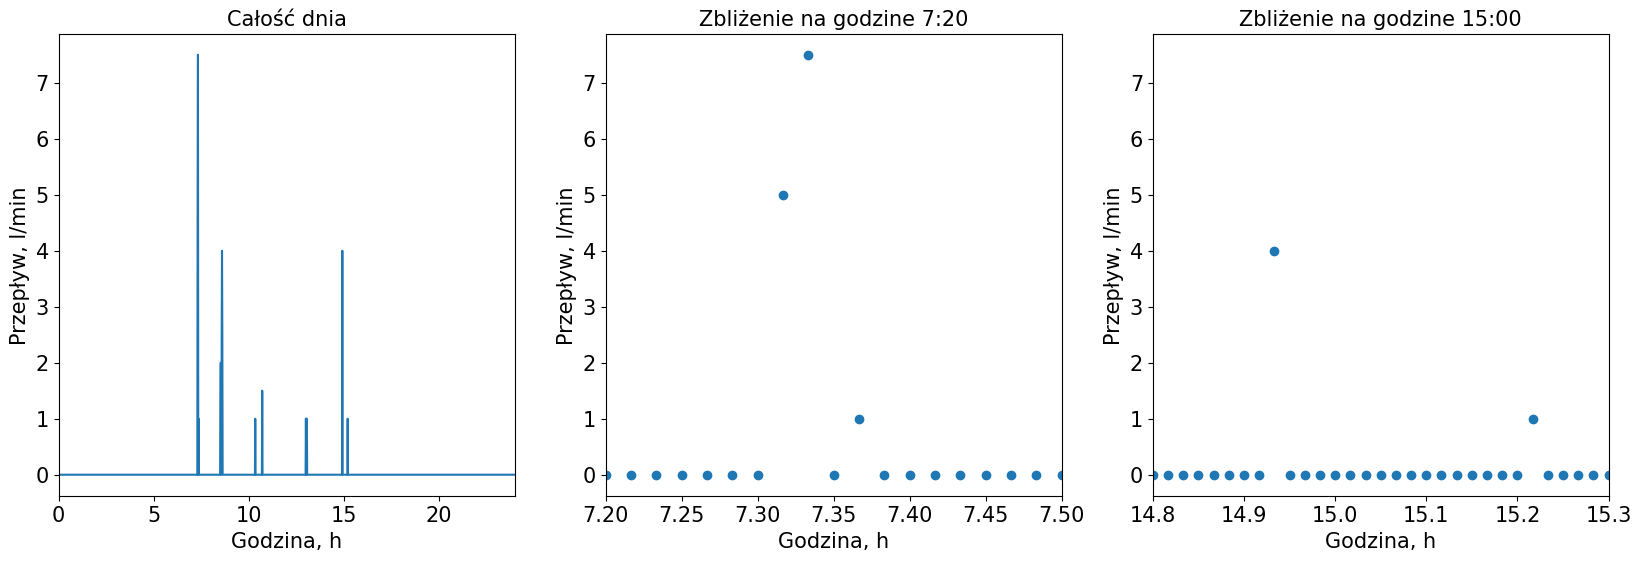
\includegraphics[width=1\textwidth]{img/Dane_nowe_disp.png}
  \caption{Podpis rysunku zawsze pod rysunkiem.}
  \label{fig:etykieta-rysunku}
\end{figure}\\
Pierwszy wykres przestawia dane zebrane z domu nr. 13 zebrane w dniu 05/02/2018. Oś X oznaczająca godzinę, począwszy od północy. Oś Y reprezentuje przepływ wody w danym momencie dnia. Wykres przedstwia nieregularne piki o nierównomiernym rozkładzie. Okresami o zwiększonym przepływie są godziny 7-13 oraz 14-15. Okresy mniejszej aktywności możemy zaobserwować w godzinach późno popołudniowych oraz nocnych. Drugi i trzeci wykres przedstawiają zbliżenie na godzinę 7 oraz 15. Dzięki zwężeniu analizowanego zakresu czasu możliwe było dokładniejsze zbadanie struktury występujących pików. Ta metoda wizualizacji ujawniła, że poszczególne piki, które na ogólnym wykresie dobowym mogły sprawiać wrażenie pojedynczych punktów, w rzeczywistości są złożone z wielu pojedynczych zdarzeń. To odkrycie jest istotne, ponieważ wskazuje na bardziej złożoną dynamikę przepływu w określonych momentach doby, co na pierwszy rzut oka mogło umknąć uwadze.\\
\newpage
W celu lepszego wstępnego zrozumienia charakterystyki analizowanego zestawu danych, niezbędne jest także szczegółowe przyjrzenie się kilku losowo wybranym domostwom.\\
\begin{figure}[!h]
  \centering
  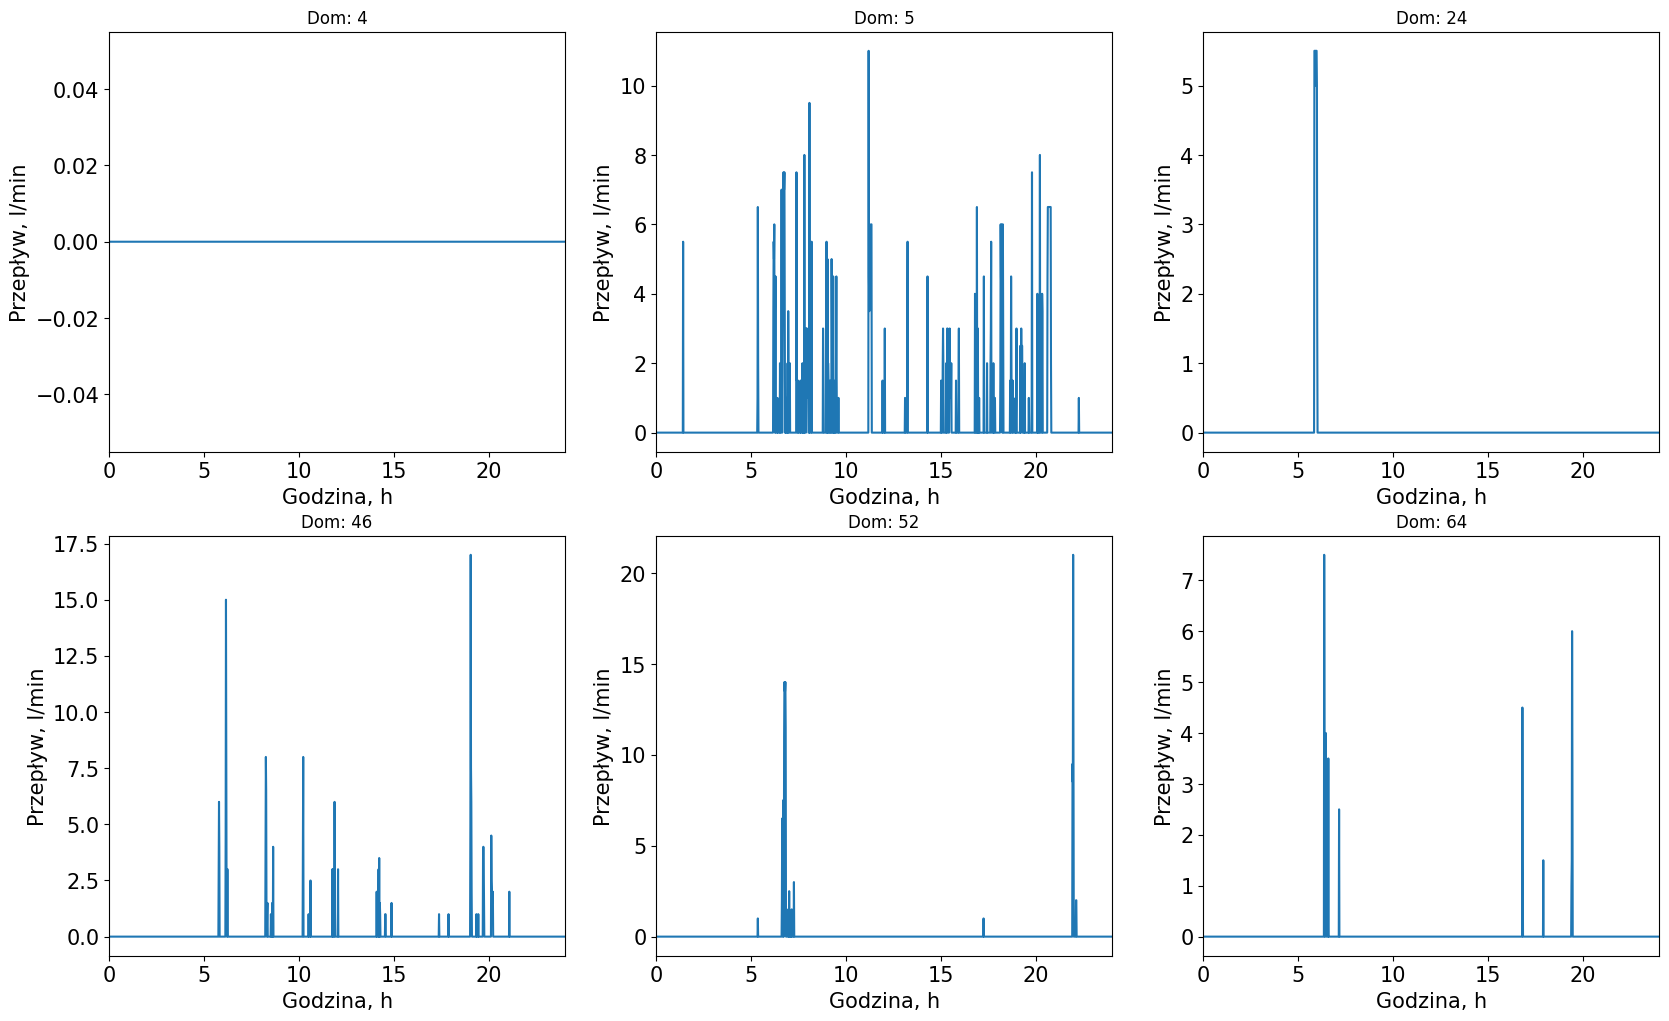
\includegraphics[width=1\textwidth]{img/Dane_nowe_compare.png}
  \caption{Porównanie przepływów dla przykładowych domów w dniu 05/02/2018}
  \label{fig:etykieta-rysunku}
\end{figure}\\
Analiza przedstawionych histogramów przepływów dla poszczególnych losowo wybranych domostw, wykonana na podstawie danych z dnia 05/02/2018, ukazuje wyraźne różnice w charakterystyce przepływów dla każdego z nich. Zgodnie z Rysunkiem 3.2, można stwierdzić, że każdy dom prezentuje unikalny wzór aktywności, co może odzwierciedlać różnorodność nawyków, planów dnia lub specyficznych potrzeb mieszkańców. Na przykład, dla domu nr 5 zużycie wody jest rozłożone przez większą część dnia, z obserwowaną aktywnością w rozmaitych godzinach. Jednakże zarejestrowano również pojedyncze zużycie w nocy. Z kolei Dom 52 charakteryzuje się wyraźnym szczytem wieczornym, co stanowi kontrast w stosunku do pozostałych domów.\\W przypadku Domu nr 4, nie odnotowano żadnego przepływu w analizowanym dniu. Brak danych może wynikać z co najmniej dwóch potencjalnych przyczyn. Pierwszą z nich jest zastosowany czas próbkowania, który wynosił jedną minutę. Taki interwał może nie być wystarczająco krótki, aby zarejestrować sporadyczne lub krótkotrwałe zdarzenia przepływu. Drugą możliwością, która może wyjaśniać brak zarejestrowanej aktywności, jest potencjalna nieobecność mieszkańców w domu w danym dniu.

\newpage
Pomimo iż zgromadzone dane charakteryzowały się wysoką jakością, ich specyficzny format wymagał przygotowania skryptu celem ich przetwarzania i ekstrakcję istotnych informacji.\\
\begin{figure}[!h]
  \centering
  \lstinputlisting[language=Python]{kod/Przetwarzanie_nowe_dane.py}
  \caption{Fragment skryptu przetwarzającego dane.}
  \label{fig:pseudokod:listings}
\end{figure}

W ramach procesu dostowania formatu aby przystosować go do wymagań tensorflow dzień tygodnia został zamieniona na etykietę liczbową, która przyjmuje wartość od 1 do 7, co odpowiada kolejnym dniom tygodnia. Podobny proces został zastosowany do etykietowania pór roku. Każda została zakodowana jako etykieta w zakresie od 1 do 4 co prezentuje kolejno wiosnę, lato, jesień i zimę. Dodatkowo czas dnia został zmieniony na procent dnia w skali od 0 do 1.
\section{Projektowanie i ocena modeli}
W ramach realizacji badań nad optymalizacją architektury sieci neuronowej oraz doborem hiperparametrów zdecydowano się na podział danych uczących na trzy zbiory. Pierwszy z nich to zestaw który zawiera dane pochodzące z 12 losowo wybranych domostw, co ma na celu zapewnienie reprezentatywności i różnorodności w ramach próby badawczej. Drugi zestaw stanowi podzbiór zawierający dane z pojedynczego gospodarstwa domowego, co pozwala na szczegółową analizę wydajności modelu w warunkach bardziej jednorodnych danych. Dodatkowo, utworzony został trzeci zestaw danych, który obejmował informacje z wszystkich 77 domów biorących udział w badaniu.


Podział zbioru danych na trzy zestawy okazał się kluczowy dla efektywnego doboru hiperparametrów modelu, szczególnie biorąc pod uwagę, że cały zbiór danych zawierał aż 12,5 miliona wierszy. Zestaw wybranych domostw, zawierający blisko 2 miliony wierszy, oraz pojedyncze domostwo z 161 tysiącami wierszy, umożliwiły przeprowadzenie dokładniejszych i bardziej zróżnicowanych testów.

Czas uczenia sieci był znacząco różny dla poszczególnych zestawów danych. Przykładowo, dla całego zbioru danych proces uczenia trwający 10 epok przy rozmiarze partii równym 64 zajmował około 46 minut. Tymczasem dla wybranych domostw czas ten skracał się do 9 minut, a dla pojedynczego domostwa uczenie trwało zaledwie 40 sekund. W ramach badań podjęto próby wykorzystania Google Colab, będącego popularnym narzędziem służącym do programowania i przetwarzania danych w chmurze. Po odpowiednim skonfigurowaniu środowiska napotkano na pierwszy znaczący problem - czas trwania uploadu pliku. Zaskakująco, przesyłanie pliku o rozmiarze 300 MB, zawierającego 12,5 miliona wierszy, zajęło znacznie więcej czasu, niż można było przewidywać. Kolejnym krokiem było przeprowadzenie procesu uczenia maszynowego na danych, zaplanowanego na 10 epok. Niestety, cały proces trwał ponad 100 minut, co wskazuje na ograniczenia wersji darmowej Google Colab. W związku z tym stwierdzono, że bez inwestycji w wersję płatną, Google Colab nie zapewnia oczekiwanej redukcji czasu niezbędnego do nauki modelu\\

Początkowo hiperparametry były testowane na najmniejszym zbiorze, co pozwalało na szybką i efektywną ocenę różnych konfiguracji. Po uzyskaniu zadowalających wyników na zbiorze pojedynczego domostwa testy były rozszerzane kolejno na zbiór wybranych domostw, a następnie na pełny zbiór danych. Taka strategia pozwoliła na stopniowe i metodyczne dostosowywanie hiperparametrów, minimalizując przy tym czas i zasoby potrzebne do przeprowadzenia eksperymentów, a jednocześnie maksymalizując ogólną skuteczność modelu. Na podstawie serii przeprowadzonych testów dotyczących dostrajania modelu wybrano następujące hiperparametry
\begin{table}[!h]
  \centering
  \caption{Hiperparametry Sieci Neuronowej}
  \begin{tabular}{|c|c|c|c|}
    \hline
    Optymalizator & Funkcja strat & Początkowy współczynnik uczenia & Rozmiar partii \\ \hline
    Adam          & mse           & 0.0001                          & 64             \\ \hline
  \end{tabular}
\end{table}

Po przeprowadzeniu serii eksperymentów, w procesie selekcji optymalnej architektury sieci neuronowej, najbardziej efektywną konfiguracją okazała się struktura składająca się z sześciu warstw, z których cztery pełniły funkcję warstw ukrytych. W procesie iteracyjnego dostosowywania i ewaluacji różnych architektur sieci, model o takiej budowie wykazał najlepsze wyniki w zakresie dokładności i generalizacji na testowanych zbiorach danych. Architektura ta charakteryzowała się kolejno malejącą liczbą neuronów w poszczególnych warstwach: pierwsza warstwa zawierała 512 neuronów, druga 256, trzecia 128, czwarta 64, piąta 32, a szósta, będąca warstwą wyjściową, miała 1 neuron. Wszystkie warstwy, z wyjątkiem ostatniej, wykorzystywały funkcję aktywacji ReLU. Natomiast ostatnia warstwa, pełniąca rolę warstwy wyjściowej, zastosowała funkcję aktywacji typu 'linear'


W ramach opracowanego modelu sieci neuronowej zastosowano dynamicznie zmieniający się współczynnik uczenia, oparty na metodzie wykładniczego spadku, opisanego wzorem:
\begin{equation}
  \text{Wspołczynik uczenia}(epoka) =
  \begin{cases}
    \text{Początkowy wspołczynik uczenia}                 & \text{jeżeli } epoka < 5    \\
    \text{Wspołczynik uczenia}(epoka - 1) \times e^{-0.1} & \text{jeżeli } epoka \geq 5
  \end{cases}
\end{equation}
Użycie tej motody pozwoliło na zmniejszanie wartości współczynnika uczenia w trakcie procesu trenowania, co zwiększyło zdolności adaptacyjne sieci. Został on zastosowany, gdyż częstym zjawiskiem było generowanie przez sieć stałej wartości wyjściowej, niezależnie od różnych danych wejściowych.

W ramach procesu testowania różnych konfiguracji sieci neuronowej zaproponowano eksplorację wydajności modeli przy różnorodnych kombinacjach wejść. Celem tego podejścia było zbadanie, jak zmiana danych wejściowych wpłynie na zdolność modelu do nauki i generalizacji przewidywania przepływu. Poniżej przedstawiono zestawienie modeli, które zostały uwzględnione w analizie:

\begin{enumerate}
  \item Model A
        \begin{enumerate}
          \item Wejścia: Dzień tygodnia, pora dnia
          \item Wyjście: Przepływ
        \end{enumerate}
  \item Model B
        \begin{enumerate}
          \item Wejścia: pora dnia
          \item Wyjście: Przepływ
        \end{enumerate}
  \item Model C
        \begin{enumerate}
          \item Wejścia: pora roku, dzień tygodnia, pora dnia
          \item Wyjście: Przepływ
        \end{enumerate}
  \item Model D
        \begin{enumerate}
          \item Wejścia: pora roku, pora dnia
          \item Wyjście: Przepływ
        \end{enumerate}
\end{enumerate}

Wyniki te dostarczą wglądu w to, które wejścia są najbardziej wartościowe dla modelowania przepływu oraz czy dodanie dodatkowych informacji kontekstowych przyczynia się do znaczącej poprawy wyników predykcyjnych.
\newpage

\section{Walidacja i próby dostrajania (?)}
W celu weryfikacji poprawności i efektywności opracowanego modelu sieci neuronowej przeprowadzono porównanie modelu nauczonych na danych ze wszystkich 12 domostw z modelami utworzonymi dla każdego z tych domów osobno. Taki eksperyment miał na celu ocenę zdolności generalizacji modelu nauczonych na zbiorze 12 domostw w porównaniu z modelami specyficznymi dla poszczególnych domów.

\begin{figure}[!h]
  \centering
  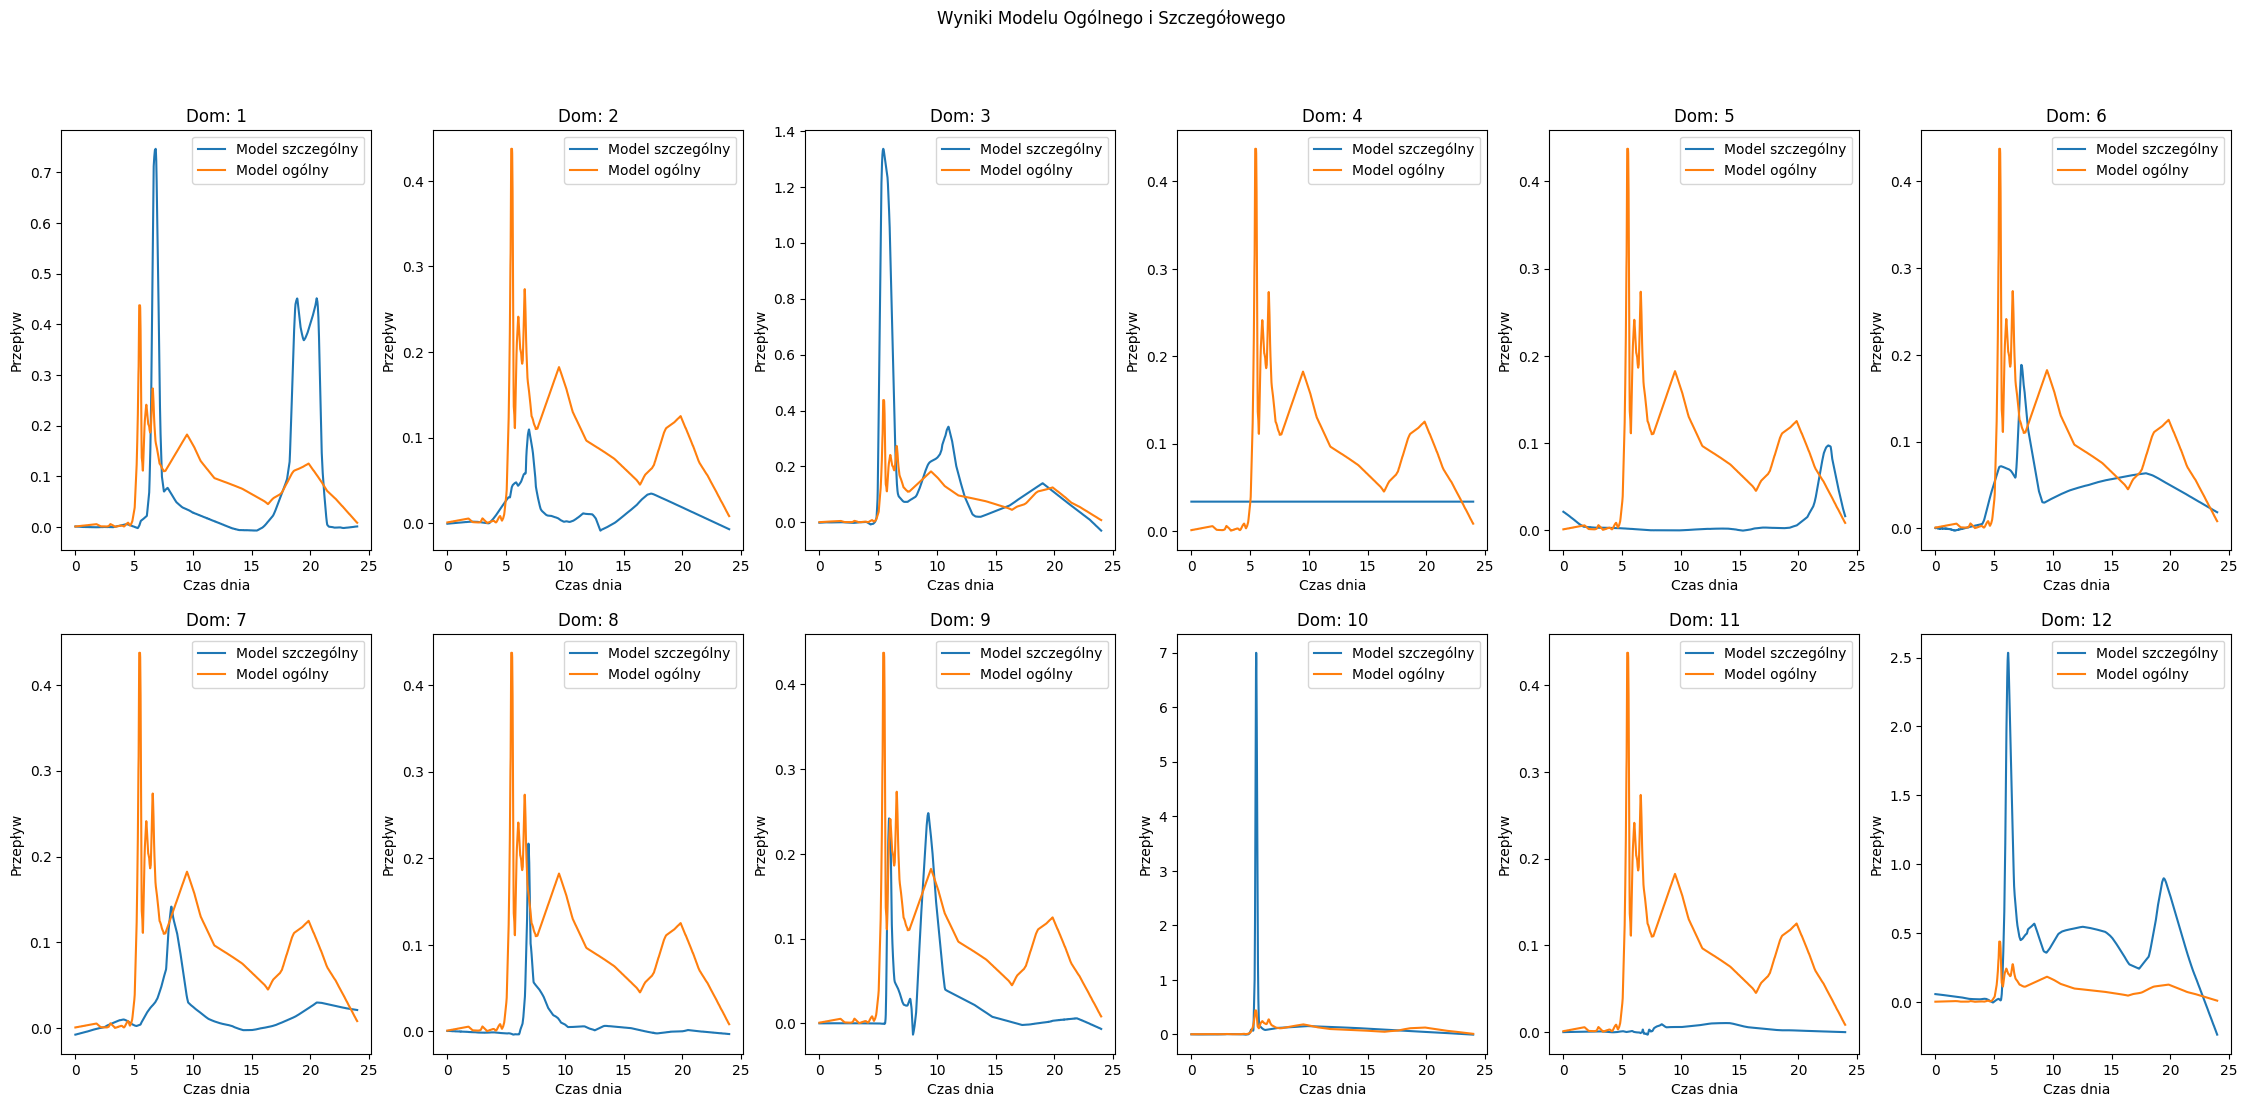
\includegraphics[width=1\textwidth]{img/szczegółowy_ogolny_porówniaie.png}
  \caption{Porównianie modelu ogólnego z modelami szczególnymi}
  \label{fig:etykieta-rysunku}
\end{figure}

W celu dalszego zwiększenia skuteczności modelu sieci neuronowej zaproponowano wprowadzenie dodatkowego wejścia do systemu – tygodniowego zużycia. Implementacja tego rozwiązania została przeprowadzona w specyficzny sposób, mający na celu uniknięcie przekształcenia tego parametru w niezamierzony label identyfikujący poszczególne domy. W fazie uczenia modelu, do każdego tygodnia przypisywano sumę zużycia zarejestrowanego w tym okresie. Natomiast w fazie testowania, model otrzymywał średnią wartość tygodniowego zużycia. Celem tej strategii było umożliwienie modelowi korzystania z danych historycznych zużycia w sposób, który poprawiałby jego zdolność do przewidywania, jednocześnie zachowując elastyczność i możliwość generalizacji wyników na różne domostwa.

\newpage

\begin{figure}[!h]
  \centering
  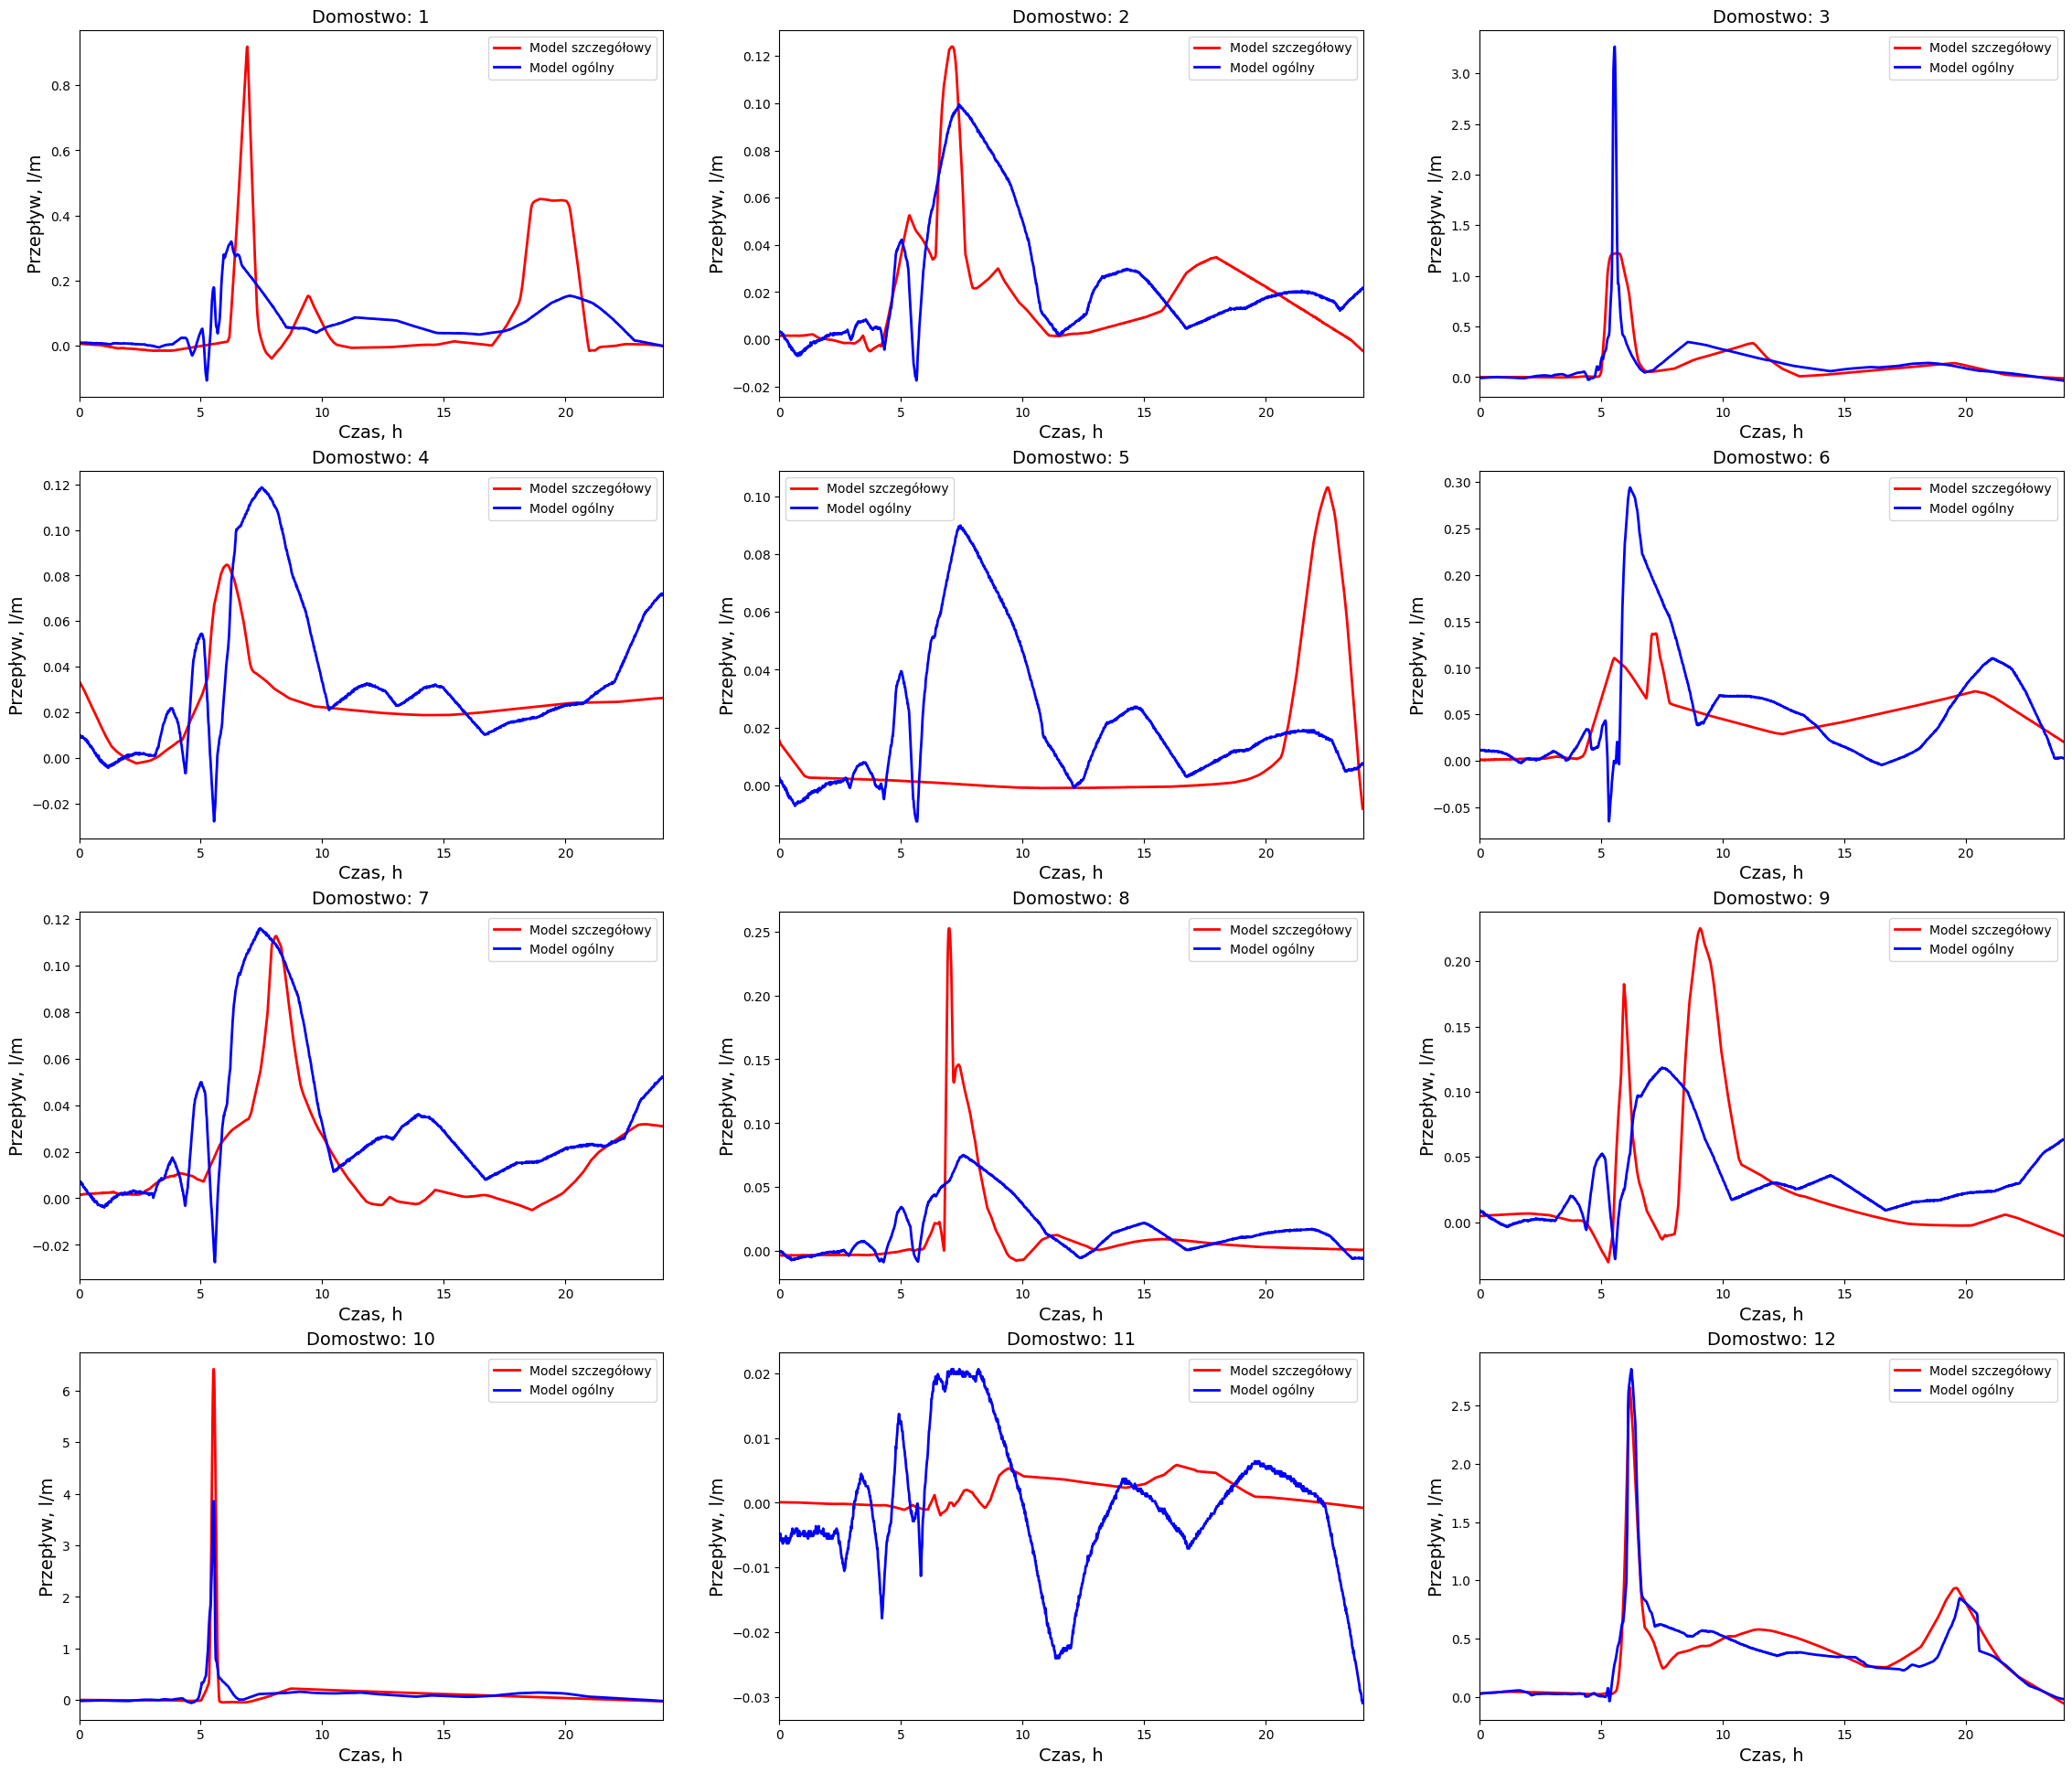
\includegraphics[width=1\textwidth]{img/szczegółowy_ogolny_porówniaie_dodatkowy.png}
  \caption{Porównianie modelu ogólnego z modelami szczególnymi po dodaniu kolejnego wejścia do sieci}
  \label{fig:etykieta-rysunku}
\end{figure}

Analizując charakterystykę modelu ogólnego i szczególnego dla każdego z domostw, przedstawioną na Rysunku 3.5, można zauważyć, że dla domostwa nr 10 i 12 model ogólny wykazał się wysoką zgodnością z modelem szczegółowym, co świadczy o jego zdolności do precyzyjnego odwzorowania charakterystyki przewidywania przepływu w ciągu dnia. W przypadku tych dwóch domów przebieg przewidywań dla obu modeli jest podobny, co wskazuje na to, że model ogólny efektywnie uchwycił dynamikę zużycia charakterystyczną dla tych konkretnych domostw. Natomiast w kontekście Domu nr 5, wyniki ukazują, że model ogólny miał znaczne trudności z dopasowaniem się do wzorców przepływu.

W celu dokładniejszej oceny i porównania efektywności modelu ogólnego, nauczonego na danych z 12 domostw, z modelami szczegółowymi, nauczonymi dla poszczególnych domów, zastosowano wskaźnik błędu średniokwadratowego. MSE, obliczany jako średnia kwadratów różnic między wartościami przewidywanymi przez model a rzeczywistymi danymi, posłużył jako miara odchylenia modelu ogólnego od wyników modeli szczegółowych. W tym kontekście niższa wartość MSE wskazywała na lepszą zgodność modelu ogólnego z wynikami modeli szczegółowych, sugerując, że model ogólny skuteczniej generalizuje dane, zbliżając się do precyzji modeli trenowanych na danych z pojedynczych domostw.

\begin{table}[!h]
  \centering
  \caption{Porównianie wartości MSE dla każdego obu modelów}
  \resizebox{\textwidth}{!}{
    \begin{tabular}{|c|cccccccccccc|}
      \hline
      \multirow{2}{*}{MSE} & \multicolumn{12}{c|}{DOMOSTWO}                                                                                                                                                                                                                                                                                                                        \\ \cline{2-13}
                           & \multicolumn{1}{c|}{1}         & \multicolumn{1}{c|}{2}       & \multicolumn{1}{c|}{3}     & \multicolumn{1}{c|}{4}       & \multicolumn{1}{c|}{5}      & \multicolumn{1}{c|}{6}      & \multicolumn{1}{c|}{7}       & \multicolumn{1}{c|}{8}       & \multicolumn{1}{c|}{9}      & \multicolumn{1}{c|}{10}    & \multicolumn{1}{c|}{11}      & 12    \\ \hline
      Model 1              & \multicolumn{1}{c|}{0.022}     & \multicolumn{1}{c|}{0.0074}  & \multicolumn{1}{c|}{0.037} & \multicolumn{1}{c|}{0.0067}  & \multicolumn{1}{c|}{0.011}  & \multicolumn{1}{c|}{0.0039} & \multicolumn{1}{c|}{0.0084}  & \multicolumn{1}{c|}{0.0095}  & \multicolumn{1}{c|}{0.0072} & \multicolumn{1}{c|}{0.22}  & \multicolumn{1}{c|}{0.010}   & 0.19  \\ \hline
      Model 2              & \multicolumn{1}{c|}{0.019}     & \multicolumn{1}{c|}{0.00053} & \multicolumn{1}{c|}{0.034} & \multicolumn{1}{c|}{0.00085} & \multicolumn{1}{c|}{0.0013} & \multicolumn{1}{c|}{0.0025} & \multicolumn{1}{c|}{0.00055} & \multicolumn{1}{c|}{0.00069} & \multicolumn{1}{c|}{0.0027} & \multicolumn{1}{c|}{0.075} & \multicolumn{1}{c|}{0.00013} & 0.019 \\ \hline
    \end{tabular}
  }
\end{table}

Analizując przedstawione dane w tabeli, można zauważyć, że po dodaniu dodatkowego wejścia do systemu, czyli tygodniowego zużycia, model 2 (Model z dodatkowym wejściem) osiągnął znacznie lepsze wyniki w porównaniu z modelem bazowym. Wartości błędu średniokwadratowego dla modelu 2 są niższe w porównaniu do modelu 1 dla każdego z domostw, co wskazuje na poprawę dokładności predykcji.
Na przykład, dla Domu nr 2, MSE zmniejszyło się z 0.0074 w modelu 1 do 0.00053 w modelu 2, co jest znaczącą poprawą. Podobne znaczące redukcje można zaobserwować w przypadku Domu nr 12, gdzie MSE spadło z 0.19 do 0.019


\chapter{Pogoda}
\label{ch:0X}

NAPISAĆ TUTAJ COŚ!\\

\begin{figure}[!h]
  \centering
  \includegraphics[width=1\textwidth]{img/Pogoda_porównanie.png}
  \caption{Porównanie warunkuch atmosferycznych na przestrzeni dnia}
  \label{fig:etykieta-rysunku}
\end{figure}
Rysunek przedstawia zestaw sześciu wykresów, które porównują warunki atmosferyczne w ciągu dnia. Każdy wykres zawiera oś X, która reprezentuje czas, oraz oś Y, która przedstawia różne zmienne meteorologiczne. W pierwszym wykresie prezentowane są zmiany temperatury zewnętrznej na przestrzeni dnia. Temperatura oscyluje w zakresie od około -0.5°C do 2.5°C, z maksymalnymi wartościami obserwowanymi w okolicach godziny ósmej. Charakterystyka tej zmienności temperatury sugeruje, że dane mogły być zbierane w okresie zimowym. Następny wykres ilustruje zmiany wilgotności powietrza na zewnątrz budynku, wyrażone w procentach. Wysoki poziom wilgotności, utrzymujący się przez cały dzień, może wskazywać na sezon zimowy lub jesienny. Prędkość wiatru, prezentowana na kolejnym wykresie, wykazuje znaczący wzrost w ciągu dnia, osiągając maksymalne wartości przekraczające 8  $\frac{m}{s}$, co może być charakterystyczne dla warunków zimowych, kiedy wiatry są silniejsze. Wykres ciśnienia atmosferycznego pokazuje wzrost wartości w pierwszej połowie dnia, po czym następuje stopniowy spadek. Wilgotność wewnętrzna, prezentowana na piątym wykresie, wykazuje wahania z ogólnym trendem spadkowym w drugiej połowie dnia. Szósty wykres przedstawia kierunek wiatru, który jest zmienny w ciągu dnia, z wyraźnymi zmianami szczególnie w środkowej części dnia, co może świadczyć o niestabilnych warunkach atmosferycznych.\\

W celu zbadania wpływu wielkości modelu na wyniki oraz sprawdzenia ważności różnych wejść, zaproponowano w badaniu dwa modele o różnej złożoności architektury. Oba modele korzystały z tej samej funkcji harmonogramowania tempa uczenia, która redukowała szybkość uczenia po czwartej epoce, oraz z tych samych parametrów kompilacji, w tym optymalizatora Adam z początkową szybkością uczenia 0.001, funkcji straty MSE
Pierwszy model składał się z mniejszej liczby warstw i neuronów: warstwa normalizująca, trzy warstwy gęste z odpowiednio 64, 32 i 1 neuronami, używając funkcji aktywacji 'relu' dla pierwszych dwóch warstw i 'linear' dla warstwy wyjściowej.
Drugi model był znacznie większy, zawierając więcej warstw i neuronów: warstwa normalizująca, sześć warstw gęstych o zwiększającej się liczbie neuronów: 1024, 512, 256, 128, 64, 32, zakończonych warstwą wyjściową z 1 neuronem, używając funkcji aktywacji 'relu' dla warstw ukrytych i 'linear' dla warstwy wyjściowej.
Oba modele były trenowane przez 50 epok z rozmiarem partii równym 32. Celem porównania tych dwóch modeli było ustalenie, czy zwiększenie liczby warstw i neuronów w modelu wpłynie na jego

W ramach procesu weryfikacji skuteczności zastosowanych modeli sieci neuronowych została zastosowana walidacja krzyżowa, metodą holdout. Dane zostały podzielone w proporcji 80\% do 20\% na zestaw treningowy i testowy. Ta strategia podziału danych miała na celu zapewnienie solidnej bazy do nauki modeli oraz efektywnej oceny ich wydajności. Model numer 1 wykazał się niższą skutecznością w porównaniu do modelu numer 2. Świadczy o tym wartość błędu średniokwadratowego, która dla modelu pierwszego wyniosła 0.0668, natomiast dla modelu drugiego było to znacząco niższe, a mianowicie 0.0237. Ta różnica w wartościach MSE wskazuje na wyższą precyzję i efektywność modelu numer 2 w procesie uczenia i oceny na podstawie dostępnych danych.
\newpage
\section{Permutacyjna Ważność Cech}
Permutacyjna Ważność Cech, to technika stosowana w uczeniu maszynowym do oceny znaczenia poszczególnych wejść dla modelu predykcyjnego. Metoda ta jest stosowana zarówno dla modeli klasyfikacyjnych, jak i regresyjnych. Proces ten rozpoczyna się od trenowania modelu na oryginalnym zestawie danych, co pozwala na ustalenie bazowej wydajności modelu. Następnie przeprowadza się permutację każdej cechy z osobna w zbiorze testowym, losowo mieszając jej wartości, podczas gdy wszystkie inne cechy pozostają niezmienione. Po dokonaniu permutacji model jest ponownie oceniany na zmodyfikowanym zbiorze danych. Wyniki tej oceny są następnie porównywane z wynikami uzyskanymi na oryginalnym, niezmodyfikowanym zbiorze. Różnica w wydajności modelu, taka jak spadek dokładności w klasyfikacji lub wzrost błędu średniokwadratowego w regresji, jest wykorzystywana do oceny ważności danej cechy. Im większy spadek wydajności, tym większa uważana jest ważność tej cechy dla modelu.

W kontekście wykorzystania PFI do oceny ważności cech w modelu istotne jest zwrócenie uwagi na kwestię korelacji między danymi. PFI opiera się na permutacji pojedynczych cech, co oznacza zmianę wartości jednej zmiennej niezależnie od pozostałych. W przypadku, gdy dane są silnie skorelowane, taka metoda permutacji może prowadzić do błędnych wniosków

W celu implementacji techniki PFI w pracy został wykorzystany obiekt PermutationImportance z biblioteki sklearn. Zastosowanie tego dedykowanego narzędzia umożliwiło nie tylko dokładną, ale i wydajną realizację tej metody, co pozwoliło na jej skuteczną integrację z procesem badawczym.

\begin{table}[!h]
  \centering
  \caption{Porównianie ważności wejść dla metody PFI}
  \resizebox{\textwidth}{!}{
    \begin{tabular}{|c|c|c|c|c|c|c|}
      \hline
                   & \begin{tabular}[c]{@{}c@{}}Temperatura \\ zewnętrzna\end{tabular} & \begin{tabular}[c]{@{}c@{}}Wilgotność\\  zewnętrzna\end{tabular} & \begin{tabular}[c]{@{}c@{}}Ciśnienie\\  atmosferyczne\end{tabular} & \begin{tabular}[c]{@{}c@{}}Prędkość\\  wiatru\end{tabular} & \begin{tabular}[c]{@{}c@{}}Kierunek\\  wiatru\end{tabular} & \begin{tabular}[c]{@{}c@{}}Wilgotność \\ wewnętrzna\end{tabular} \\ \hline
      Model krótki & 0.48                                                              & 1.00                                                             & 0.39                                                               & 0.07                                                       & 0.03                                                       & 0.36                                                             \\ \hline
      Model długi  & 0.47                                                              & 0.11                                                             & 0.65                                                               & 0.23                                                       & 0.17                                                       & 1.00                                                             \\ \hline
    \end{tabular}
  }
\end{table}
Tabela 4.1 porównuje znormalizowane wartości wejść dla dwóch wariantów modelu dla metody PFI, w modelu uproszczonym, najwyższą ważność ma wilgotność zewnętrzna, co sugeruje, że jest to główny predyktor w tym modelu. Temperatura zewnętrzna i wilgotność wewnętrzna również odgrywają znaczące role. Wilgotność zewnętrzna mają umiarkowaną ważność, podczas gdy kierunek i prędkość wiatru ma stosunkowo niższą ważność. W Modelu rozszerzonym obserwujemy wzrost ważności ciśnienia atmosferycznego. Interesująco, wilgotność wewnętrzna otrzymuje maksymalną ważność, co czyni ją najważniejszą cechą dla tego modelu, z kolei prędkość i kierunek wiatru mają większy wpływ w porównaniu do Modelu krótkiego. Wilgotność zewnętrzna doznaje znaczącego obniżenia ważności, zostajac cechą o najniższej wartości.
\newpage
\section{Badanie wag wejściowych pierwszej warsty}
W analizie modeli uczenia maszynowego, interpretacja wag pierwszej warstwy może służyć jako metoda określania ważności cech wejściowych. Ponieważ wagi w pierwszej warstwie sieci neuronowej są bezpośrednio połączone z cechami wejściowymi, wartości tych wag mogą dostarczać informacji o znaczeniu poszczególnych cech dla predykcji modelu. Wysoka wartość wagowa sugeruje, że zmiana wartości tej cechy wejściowej może mieć istotny wpływ na wynik modelu. Jednakże, ta metoda interpretacji może być mniej efektywna w przypadku bardziej złożonych, głębokich sieci neuronowych. W takich modelach, liczne warstwy i skomplikowane struktury, w tym nieliniowe aktywacje i interakcje między neuronami, mogą skutkować tym, że bezpośredni wpływ pojedynczych wag jest trudniejszy do zrozumienia.
\begin{figure}[!h]
  \centering
  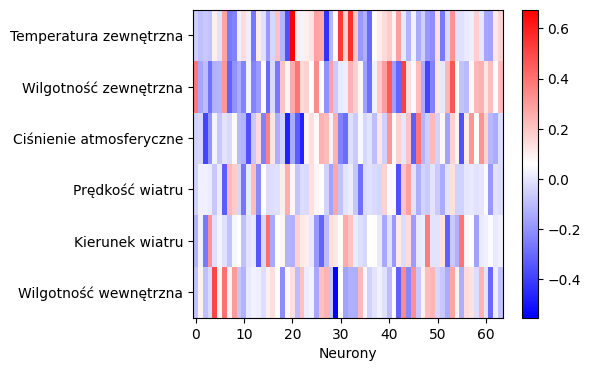
\includegraphics[width=0.7\textwidth]{img/heatmap1.png}
  \caption{Mapa ciepła wag pierwszej warstwy dla modelu o uproszczonej architekturze}
  \label{fig:etykieta-rysunku}
\end{figure}

Mapa ciepła wag pierwszej warstwy sieci neuronowej stanowi cenne narzędzie analityczne, pozwalające na wizualną interpretację i zrozumienie wpływu dużej liczby cech na proces uczenia. Jest to instrument szczególnie użyteczny w kontekście wysokowymiarowych zbiorów danych, gdzie tradycyjne metody analizy mogą okazać się niewystarczające. W przedstawionym przypadku, analiza mapy ciepła nie ujawnia istotnych anomalii w rozkładzie wag. Obserwuje się jedynie sporadyczne wartości, które odstają od średnich wag, lecz nie osiągają one poziomu znacząco wpływającego na wyniki modelu.

W celu dokładnej analizy ważności poszczególnych wag wejściowych sieci neuronowej przeprowadzono obliczenie średniej wartości wagi dla każdego z wejść. Procedura ta umożliwiła identyfikację względnej ważności cech poprzez porównanie ich przeciętnego wpływu na aktywację neuronów w modelu. Następnie, aby umożliwić porównywalność wyników niezależnie od ich pierwotnej skali, dokonano normalizacji obliczonych średnich wag.
\begin{table}[!h]
  \centering
  \caption{Porównianie wag wejściowych dla pierwszej warstwy uproszczonego modelu}
  \resizebox{\textwidth}{!}{
    \begin{tabular}{|c|c|c|c|c|c|}
      \hline
      \begin{tabular}[c]{@{}c@{}}Temperatura \\ zewnętrzna\end{tabular} & \begin{tabular}[c]{@{}c@{}}Wilgotność\\  zewnętrzna\end{tabular} & \begin{tabular}[c]{@{}c@{}}Ciśnienie\\  atmosferyczne\end{tabular} & \begin{tabular}[c]{@{}c@{}}Prędkość\\  wiatru\end{tabular} & \begin{tabular}[c]{@{}c@{}}Kierunek\\  wiatru\end{tabular} & \begin{tabular}[c]{@{}c@{}}Wilgotność \\ wewnętrzna\end{tabular} \\ \hline
      0.92                                                              & 0.48                                                             & 1.00                                                               & 0.56                                                       & 0.53                                                       & 0.40                                                             \\ \hline
    \end{tabular}
  }
\end{table}\\

Analiza ważności wejść pierwszej warstwy sieci neuronowej, przeprowadzona za pomocą metody badania wag wejściowych, ujawnia istotne różnice w porównaniu z wynikami uzyskanymi metodą Permutation Feature Importance dla modelu o mniej rozbudowanej architekturze. W przeprowadzonych badaniach największą ważność przyznano ciśnieniu atmosferycznemu, co stanowi odchylenie od wyników w wynikach PFI.

Dodatkowo, warto zauważyć, że w badaniu wag wejściowych pierwszej warstwy, temperatura zewnętrzna otrzymała ważność równą 0.92, co jest wynikiem świadczącym o jej istotnym wpływie na model. Jest to wartość znacznie przewyższająca inne cechy, co sugeruje, że temperatura zewnętrznai ciśnienie atmosferyczne pełnią dominującą rolę w przewidywaniach modelu. W kontraście do nich, wilgotność zewnętrzna, prędkość wiatru oraz kierunek wiatru uzyskały ważności w okolicach 0.5, co wskazuje na ich umiarkowany, lecz w miarę zrównoważony wkład w działanie modelu.

Z kolei kierunek wiatru został oceniony jako cecha o najniższej ważności w badaniu wag wejściowych, jednakże nawet ta najniższa wartość (0.4) jest znacznie wyższa niż najniższe ważności zarejestrowane w metodzie PFI, gdzie dla wilgotności wewnętrznej odnotowano wartość minimalną na poziomie 0.03. Jest to szczególnie godne uwagi, gdyż wskazuje to na różnice w interpretacji znaczenia poszczególnych cech w zależności od zastosowanej metody analizy ważności wejść.\\

Analizy bardziej złożonych modeli sieci neuronowych, metoda interpretacji wag pierwszej warstwy może okazać się nieefektywna. Ze względu na zwiększoną głębokość i złożoność architektury, wagi w pierwszej warstwie tracą bezpośrednią i jednoznaczną interpretowalność, która jest charakterystyczna dla prostszych modeli. W modelach rozbudowanych, cechy wejściowe przechodzą przez wiele warstw transformacji, co skutkuje utratą bezpośredniego powiązania między wagami pierwszej warstwy a wynikowymi decyzjami modelu. W efekcie, interpretacja tych wag może nie odzwierciedlać faktycznego wpływu poszczególnych cech na decyzje modelu, co jest spowodowane nakładaniem się, transformacją i połączeniem informacji w kolejnych warstwach sieci.
\newpage
\begin{figure}[!h]
  \centering
  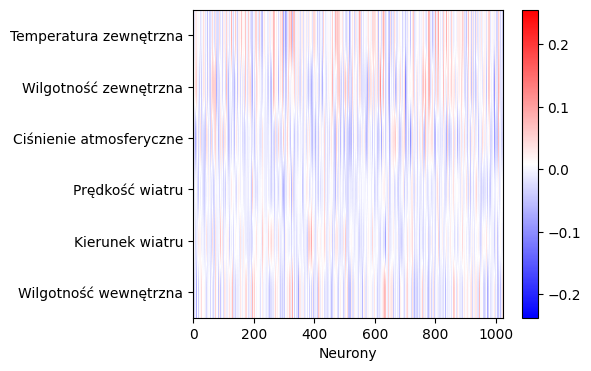
\includegraphics[width=0.6\textwidth]{img/heatmap2.png}
  \caption{Mapa ciepła wag pierwszej warstwy dla modelu o rozbudowanej architekturze}
  \label{fig:etykieta-rysunku}
\end{figure}

Na przedstawionej mapie cieplnej, ilustrującej wagi przypisane poszczególnym neuronom w warstwie wejściowej sieci neuronowej o rozmiarze 1024 jednostek, zaobserwować można istotne wzorce, choć sama mapa staje się trudna do interpretacji ze względu na dużą gęstość neuronów. Mimo tej wizualnej złożoności, zauważyć można, że temperatura zewnętrzna jest reprezentowana przez znacząco większą liczbę wag o dodatnich wartościach. W przeciwieństwie, ciśnienie atmosferyczne wykazuje tendencję do posiadania większej ilości wag o wartościach ujemnych. Wagi odpowiadające kierunkowi wiatru wydają się charakteryzować przewagą wartości bliskich zeru, co sugeruje mniejszy wpływ tej cechy na model.

\begin{table}[!h]
  \centering
  \caption{Porównianie wag wejściowych dla pierwszej warstwy rozbudowanego modelu}
  \resizebox{\textwidth}{!}{
    \begin{tabular}{|c|c|c|c|c|c|}
      \hline
      \begin{tabular}[c]{@{}c@{}}Temperatura \\ zewnętrzna\end{tabular} & \begin{tabular}[c]{@{}c@{}}Wilgotność\\  zewnętrzna\end{tabular} & \begin{tabular}[c]{@{}c@{}}Ciśnienie\\  atmosferyczne\end{tabular} & \begin{tabular}[c]{@{}c@{}}Prędkość\\  wiatru\end{tabular} & \begin{tabular}[c]{@{}c@{}}Kierunek\\  wiatru\end{tabular} & \begin{tabular}[c]{@{}c@{}}Wilgotność \\ wewnętrzna\end{tabular} \\ \hline
      1.00                                                              & 0.11                                                             & 0.75                                                               & 0.73                                                       & 0.61                                                       & 0.13                                                             \\ \hline
    \end{tabular}
  }
\end{table}

Analiza przeprowadzona z wykorzystaniem mapy cieplnej okazała się w tym przypadku być wyjątkowo efektywnym narzędziem, pozwalającym na wizualne wyodrębnienie cech o dużej wadze dla modelu. Obserwacje dotyczące tempetaru zewnętrznej i ciśnienia atmosferyznego pokrywają sie z wynikami otrzymanymi z analizy wag wejść do pierwszej warstywy. Interesującym zaskoczeniem okazała się natomiast rola kierunku wiatru, który początkowo oszacowany jako cecha mało znacząca, okazał sie znacznie znaczącym.

\newpage
\section{LIME}
W kontekście zrozumienia modeli uczenia maszynowego, metoda Local Interpretable Model-agnostic Explanations jest istotnym narzędziem, które umożliwia interpretację decyzji modelu na poziomie lokalnym. Metoda ta wyróżnia się spośród innych, takich jak PFI, dzięki swojemu unikalnemu podejściu skoncentrowanemu na pojedynczych instancjach danych. Podczas gdy PFI dąży do zapewnienia ogólnego zrozumienia wpływu cech na model przez zbieranie i analizowanie informacji z różnych instancji, LIME skupia się na wyjaśnieniu, w jaki sposób model dokonuje przewidywań dla konkretnej, wybranej próbki danych.

Podstawowym elementem metody LIME jest modyfikacja danych i tworzenie na ich podstawie uproszczonego modelu, który ma za zadanie odwzorować zachowanie oryginalnego, skomplikowanego modelu, ale tylko w ograniczonym, lokalnym obszarze wokół analizowanej instancji. Proces ten rozpoczyna się od stworzenia zbioru danych przez modyfikację wybranej instancji, co skutkuje powstaniem podobnych, ale nieidentycznych przykładów. Następnie, na tych zmodyfikowanych danych, oblicza się przewidywania za pomocą oryginalnego modelu. Kluczowym krokiem jest trenowanie prostego modelu, takiego jak regresja liniowa, na podstawie tych przewidywań. Model ten służy do aproksymacji wpływu zmian w danych na przewidywania modelu. W ten sposób, analizując współczynniki modelu liniowego, można zrozumieć, które cechy miały największy wpływ na przewidywania dla danej instancji.

W ramach pracy, w celu dokładnej oceny skuteczności metody LIME, zdecydowano się na zastosowanie jej na losowo wybranych próbkach ze zbioru testowego.

\begin{table}[!h]
  \caption{Porównanie ważności wejść dla metody LIME}
  \resizebox{\textwidth}{!}{
    \begin{tabular}{|c|c|c|c|c|c|c|}
      \hline
                                                                         & \begin{tabular}[c]{@{}c@{}}Temperatura \\ zewnętrzna\end{tabular} & \begin{tabular}[c]{@{}c@{}}Wilgotność\\  zewnętrzna\end{tabular} & \begin{tabular}[c]{@{}c@{}}Ciśnienie\\ atmosferyczne\end{tabular} & \begin{tabular}[c]{@{}c@{}}Prędkość\\ wiatru\end{tabular} & \begin{tabular}[c]{@{}c@{}}Kierunek\\ wiatru\end{tabular} & \begin{tabular}[c]{@{}c@{}}Wilgotność\\  wewnętrzna\end{tabular} \\ \hline
      \multirow{3}{*}{\begin{tabular}[c]{@{}c@{}}Model\\ 1\end{tabular}} & 0.17                                                              & 0.57                                                             & 1.00                                                              & 0.09                                                      & 0.00                                                      & 0.00                                                             \\ \cline{2-7}
                                                                         & 1.00                                                              & 0.36                                                             & 0.08                                                              & 0.04                                                      & 0.02                                                      & 0.36                                                             \\ \cline{2-7}
                                                                         & 1.00                                                              & 0.02                                                             & 0.02                                                              & 0.04                                                      & 0.00                                                      & 0.32                                                             \\ \hline
      \multirow{3}{*}{\begin{tabular}[c]{@{}c@{}}Model\\ 2\end{tabular}} & 0.33                                                              & 0.33                                                             & 0.27                                                              & 0.13                                                      & 1.00                                                      & 0.93                                                             \\ \cline{2-7}
                                                                         & 1.00                                                              & 0.10                                                             & 0.15                                                              & 0.07                                                      & 0.10                                                      & 0.10                                                             \\ \cline{2-7}
                                                                         & 1.00                                                              & 0.02                                                             & 0.19                                                              & 0.09                                                      & 0.00                                                      & 0.78                                                             \\ \hline
    \end{tabular}
  }
\end{table}

Tabela przedstawia wyniki sześciu losowo wybranych prób oceny ważności wejść, z zastosowaniem zarówno modelu uproszczonego, jak i rozszerzonego. W celu ułatwienia porównania, wyniki te zostały znormalizowane i zaokrąglone do dwóch miejsc po przecinku. Analiza danych wykazała, że w dwóch na trzy przypadki, zarówno w modelu uproszczonym, jak i rozszerzonym, najważniejszym wejściem okazała się być temperatura zewnętrzna. Ponadto, w pięciu z sześciu analizowanych przypadków, kierunek wiatru został oceniony jako najmniej znaczący.

Szczególnie interesująca jest obserwacja z pierwszej próby, gdzie temperatura zewnętrzna otrzymała znacznie niższą wagę, podczas gdy ciśnienie atmosferyczne, które zazwyczaj charakteryzowało się niższymi wagami, w tej próbie uzyskało najwyższą. Z kolei prędkość wiatru, niezależnie od zastosowanego modelu, konsekwentnie otrzymywała niską wagę w każdej z prób.\\

Mimo iż LIME jest metodą zasadniczo skoncentrowaną na dostarczaniu interpretacji lokalnych, istnieje możliwość adaptacji jej do generowania wniosków o charakterze bardziej ogólnym. Można to osiągnąć poprzez zastosowanie metody LIME wielokrotnie na różnych próbkach danych, a nastepnie wyciąganięcie średniej. Zaproponowano wybranie czterech zestawów ze zbioru testowego, zawierających odpowiednio 10, 50, 100, i 1000 próbek.


\begin{table}[!h]
  \caption{Porównanie uśrednionych ważności wejść dla metody LIME dla wielu prób}
  \resizebox{\textwidth}{!}{
    \begin{tabular}{|c|c|c|c|c|c|c|c|}
      \hline
                                                                         & \begin{tabular}[c]{@{}c@{}}Ilość\\ próbek\end{tabular} & \begin{tabular}[c]{@{}c@{}}Temperatura \\ zewnętrzna\end{tabular} & \begin{tabular}[c]{@{}c@{}}Wilgotność\\  zewnętrzna\end{tabular} & \begin{tabular}[c]{@{}c@{}}Ciśnienie\\ atmosferyczne\end{tabular} & \begin{tabular}[c]{@{}c@{}}Prędkość\\ wiatru\end{tabular} & \begin{tabular}[c]{@{}c@{}}Kierunek\\ wiatru\end{tabular} & \begin{tabular}[c]{@{}c@{}}Wilgotność\\ wewnętrzna\end{tabular} \\ \hline
      \multirow{4}{*}{\begin{tabular}[c]{@{}c@{}}Model\\ 1\end{tabular}} & 10                                                     & 0.95                                                              & 0.82                                                             & 1.00                                                              & 0.20                                                      & 0.21                                                      & 0.09                                                            \\ \cline{2-8}
                                                                         & 50                                                     & 1.00                                                              & 0.21                                                             & 0.53                                                              & 0.15                                                      & 0.03                                                      & 0.01                                                            \\ \cline{2-8}
                                                                         & 100                                                    & 1.00                                                              & 0.27                                                             & 0.53                                                              & 0.26                                                      & 0.05                                                      & 0.02                                                            \\ \cline{2-8}
                                                                         & 1000                                                   & 1.00                                                              & 0.41                                                             & 0.49                                                              & 0.15                                                      & 0.01                                                      & 0.01                                                            \\ \hline
      \multirow{4}{*}{\begin{tabular}[c]{@{}c@{}}Model\\ 2\end{tabular}} & 10                                                     & 1.00                                                              & 0.35                                                             & 0.21                                                              & 0.28                                                      & 0.11                                                      & 0.01                                                            \\ \cline{2-8}
                                                                         & 50                                                     & 1.00                                                              & 0.30                                                             & 0.52                                                              & 0.33                                                      & 0.40                                                      & 0.03                                                            \\ \cline{2-8}
                                                                         & 100                                                    & 1.00                                                              & 0.44                                                             & 0.30                                                              & 0.21                                                      & 0.16                                                      & 0.03                                                            \\ \cline{2-8}
                                                                         & 1000                                                   & 1.00                                                              & 0.41                                                             & 0.84                                                              & 0.57                                                      & 0.27                                                      & 0.05                                                            \\ \hline
    \end{tabular}
  }
\end{table}

Zarówno w Modelu 1, jak i Modelu 2, temperatura zewnętrzna jest systematycznie uznawana za cechę o największym wpływie na przewidywania modelu, co wskazuje na jej przewodnią rolę w analizowanych danych meteorologicznych. Niezmiennie wysokie wartości ważności tej zmiennej świadczą o jej dominującej pozycji w obu modelach, niezależnie od wielkości próby. Dla obu modelów, wilgotność jak i ciśnienie wykazują stabilne wartości, tylko w pojedyńczych próbach ciśnienie staja sie dominującą zmienną.
Prędkość wiatru, która generalnie otrzymuje niższe ważności, ujawnia znaczący wzrost w przypadku 1000 próbek w Modelu 2. To może wskazywać na to, że dla bardziej złożonych analiz, gdy dostępna jest większa liczba danych, prędkość wiatru zaczyna wykazywać silniejsze korelacje z wynikami modelu bardzo złożonego.Kierunek wiatru dla modelu pierwszego pozostaje cechą o niskiej ważności, lecz dla modelu rozbudowanego zystkujena znaczniu. Wilgotność wewnętrzna konsekwentnie otrzymuje najniższe wartości ważności, co wskazuje na jej marginalną rolę w procesie decyzyjnym obu modeli. Wilgotność wewnętrzna i zewnętrzna zostały zidentyfikowane jako wejścia o najmniejszym wpływie na model.

\chapter{Modelowanie zbiornika CWU}
\label{ch:05}
\section{Metodologia}
linearyzacja \cite{bib:linearyzacja} \\
inne podejścia\cite{bib:model_1,bib:model_2}
\newpage
\subsection{Model jednowarstwowy}
\begin{figure}[!ht]
  \centering
  \resizebox{0.5\textwidth}{!}{%
    \begin{circuitikz}
      \tikzstyle{every node}=[font=\LARGE]
      \draw  (8.75,13.75) rectangle (11.25,8.75);
      \draw [->, >=Stealth] (10,7.5) .. controls (10,8) and (10,8) .. (10,8.75);
      \draw [->, >=Stealth] (10,15) .. controls (11.25,15) and (11.25,15) .. (12.5,15);
      \draw [->, >=Stealth] (6.5,11.25) .. controls (7.5,11.25) and (7.5,11.25) .. (8.5,11.25);
      \draw  (5,11.25) circle (1cm);
      \node [font=\LARGE] at (5,11.25) {$Q_p$};
      \draw [](10,13.75) to[short] (10,15);
      \node [font=\LARGE] at (7.5,11.75) {$F_z, T_{zi}$};
      \draw [](10,7.5) to[short] (12.5,7.5);
      \draw [](11.5,11.25) to[short, -o] (13.25,11.25);
      \node [font=\LARGE] at (11,7.9) {$T_{wi}$};
      \node [font=\LARGE] at (12.5,11.75) {$T_{ot}$};
      \node [font=\LARGE] at (11.25,15.5) {$F_w,T_{wo}$};
    \end{circuitikz}
  }%
  \caption{Model zasobnika - pojedyńcza warstwa}
  \label{Qp}
\end{figure}

\begin{equation}
  \rho C_w V \frac{dT_{wo}}{dt} = Q_p - \rho C_w F_w (T_{wo} - T_{wi}) - \frac{\lambda A}{d} (T_{wo} - T_{ot})
\end{equation}

gdzie:
\begin{itemize}
  \item[A] Powierzchnia wymiany ciepła DO POPRAWY
  \item[d] powierzchnia wymiany ciepła DO POPRAWY
  \item[V] Objętość
  \item[$C_w$] Ciepło właściwe
  \item[$\lambda$] Wspołczynnik wymiany ciepła
  \item[$Q_p$] Ciepło systemu grzewczego
  \item[$T_{ot}$] Temperatura otoczenia
  \item[$T_{wo}$] Temepratura wyjściowa
  \item[$T_{wi}$] Temperatura wejściowa
  \item[$F_{w}$] TODO
  \item[$F_{z}$] TODO
\end{itemize}
\newpage
\subsection{Model wielowarstwowy}

\begin{figure}[!ht]
  \centering
  \resizebox{0.5\textwidth}{!}{%
    \begin{circuitikz}
      \tikzstyle{every node}=[font=\Large]
      \draw  (8.75,13.75) rectangle (11.25,8.75);
      \draw [short] (8.25,13.25) .. controls (10,13.25) and (10,13.25) .. (11.75,13.25);
      \draw [short] (8.25,12.75) .. controls (10,12.75) and (10,12.75) .. (11.75,12.75);
      \draw [short] (8.25,12.25) .. controls (10,12.25) and (10,12.25) .. (11.75,12.25);
      \draw [short] (8.25,9.25) .. controls (10,9.25) and (10,9.25) .. (11.75,9.25);
      \draw [short] (8.25,9.75) .. controls (10,9.75) and (10,9.75) .. (11.75,9.75);
      \draw [short] (8.25,10.25) .. controls (10,10.25) and (10,10.25) .. (11.75,10.25);
      \draw [->, >=Stealth] (10,14.25) .. controls (10,15.25) and (10,15.25) .. (10,16.25);
      \draw [->, >=Stealth] (6.5,12.75) .. controls (7.25,12.75) and (7.25,12.75) .. (8,12.75);
      \draw [->, >=Stealth] (6.5,9.75) .. controls (7.25,9.75) and (7.25,9.75) .. (8,9.75);
      \draw [->, >=Stealth] (12.25,11.25) .. controls (13.5,11.25) and (13.5,11.25) .. (14.5,11.25);
      \node [font=\Large] at (7,13.2) {$Q_{z1}$};
      \node [font=\Large] at (7,10.2) {$Q_{zm}$};
      \node [font=\Large] at (13.25,11.7) {$Q_s$};
      \node [font=\Large] at (10.7,15) {$Q_u$};
      \node [font=\normalsize] at (12,13.5) {$Q_{wn}$};
      \node [font=\normalsize] at (12,8.75) {$Q_{w1}$};
      \node [font=\Large] at (10,11.25) {$Q_w$};
      \node [font=\Large] at (7,11.75) {.};
      \node [font=\Large] at (7,11.5) {.};
      \node [font=\Large] at (7,11.25) {.};
      \node [font=\Large] at (11.75,11.75) {.};
      \node [font=\Large] at (11.75,11.25) {.};
      \node [font=\Large] at (11.75,10.75) {.};
    \end{circuitikz}
  }%
  \caption{Model zasobnika - wiele warstwa}
  \label{Model zasobnika - wiele warstwa}
\end{figure}

\begin{equation}
  Q_w = \sum_{m=1}^{m} Q_m - Q_u - Q_s
\end{equation}

\begin{equation}
  Q_{wn} = \sum_{n=1}^{m(n)} Q_{m(n)} - Q_{un} - Q_{sn}
\end{equation}

\begin{itemize}
  \item[$Q_m$]
  \item[$Q_w$] Ciepło całego zbiornika
  \item[$Q_{wm}$] Ciepło warstwy
  \item[$Q_u$] Ciepło upuszczające zbiornik DO POPRAWY
  \item[$Q_s$] Straty ciepła
\end{itemize}

\newpage
\begin{figure}[!ht]
  \centering
  \resizebox{0.5\textwidth}{!}{%
    \begin{circuitikz}
      \tikzstyle{every node}=[font=\Large]
      \draw  (8.75,15) rectangle (11.25,10);
      \draw [->, >=Stealth] (10,8.75) .. controls (10,9.25) and (10,9.25) .. (10,10);
      \draw [->, >=Stealth] (10,16.25) .. controls (11.25,16.25) and (11.25,16.25) .. (12.5,16.25);
      \draw [line width=1pt, ->, >=Stealth] (8.75,12.25) .. controls (8.25,12.25) and (8.25,12.25) .. (7.5,12.25);
      \draw [line width=1pt,->, >=Stealth] (7.25,14.25) .. controls (7.5,14.25) and (7.5,14.25) .. (7.75,14.25);
      \draw[, line width=1pt] (7.5,12.25) to[short] (7.25,12.25);
      \draw [line width=1pt, short] (7.75,14.25) .. controls (9,14.25) and (9,14.25) .. (10,14.25);
      \draw [line width=1pt, short] (10,14.25) .. controls (9.75,14) and (9.75,14) .. (9.5,13.75);
      \draw [line width=1pt, short] (9.5,13.75) .. controls (9.75,13.5) and (9.75,13.5) .. (10,13.25);
      \draw [line width=1pt, short] (10,13.25) .. controls (9.75,13) and (9.75,13) .. (9.5,12.75);
      \draw [line width=1pt, short] (9.5,12.75) .. controls (9.75,12.5) and (9.75,12.5) .. (10,12.25);
      \draw [line width=1pt, short] (10,12.25) .. controls (9.5,12.25) and (9.5,12.25) .. (8.75,12.25);
      \draw [short] (10,15) .. controls (10,15.5) and (10,15.5) .. (10,16.25);
      \draw [short] (10,8.75) .. controls (11.25,8.75) and (11.25,8.75) .. (12.5,8.75);
      \node [font=\Large] at (7.75,14.6) {$F_z, T_{zi}$};
      \node [font=\Large] at (11.5,16.6) {$F_w, T_{wo}$};
      \node [font=\Large] at (11.25,9.1) {$T_{wi}$};
      \draw [](13.75,13.25) to[short] (13.75,15.25);
      \draw [](6.25,15.25) to[short] (6.25,13.25);
      \draw [](6.25,13) to[short] (13.75,13);
      \draw [](13.75,13) to[short] (13.75,11.5);
      \draw[] (13.75,11.5) to[short] (6.25,11.5);
      \draw [](6.25,13) to[short] (6.25,11.5);
      \draw [](6.25,11.25) to[short] (6.25,10.25);
      \draw [](6.25,10.25) to[short] (6.25,9.75);
      \draw [](13.75,9.75) to[short] (13.75,11.25);
      \draw [](6.25,13.25) to[short] (13.75,13.25);
      \draw [](6.25,15.25) to[short] (13.75,15.25);
      \draw [](6.25,11.25) to[short] (13.75,11.25);
      \draw [](6.25,9.75) to[short] (13.75,9.75);
    \end{circuitikz}
  }%
  \caption{Trójwarstwowy model zasobnika}
  \label{Qp}
\end{figure}

\begin{equation}
  \frac{dT_{wo}^{3}}{dt} = b_1^3 F_z (T_{zi} - T_{wo}^{3}) - b_2^3 F_w (T_{wo}^{3} - T_{wo}^{2}) - b_3^4 (T_{wo}^{3} - T_{ot})
\end{equation}

\begin{equation}
  \frac{dT_{zi}}{dt} = p_1 Q_g - p_2 F_z (T_{zi} - T_{wo}^{3}) - p_3 (T_{zi} - T_{ot})
\end{equation}

\begin{equation}
  \frac{dT_{wo}^{2}}{dt} = b_1^2 F_z (T_{zi} - T_{wo}^{2}) - b_2^2 F_w (T_{wo}^{2} - T_{wo}^{1}) - b_3^2 (T_{wo}^{2} - T_{ot}) - b_4^2 (T_{wo}^{2} - T_{wo}^{1}) + b_5^2 (T_{wo}^{3} - T_{wo}^{2})
\end{equation}

\begin{equation}
  \frac{dT_{wo}^{1}}{dt} = -b_2^1 F_w (T_{wo}^{1} - T_{wi}) - b_3^1 (T_{wo}^{1} - T_{ot}) + b_5^1 (T_{wo}^{2} - T_{wo}^{1})
\end{equation}

Przedstawienie modelu warstwowego, równań stanu, pokazanie wyników symulacji modelu
\section{Wyniki symulacji}


\chapter{Optymalizacja}
\label{ch:06}
\section{Funkcja kosztów}
\begin{equation}
  G = \int p_1 Q_g \, dt
\end{equation}
\section{Funkcja komfortu}
\begin{equation}
  J = \int \left( T_{wo} - T_{wym} \right)^2 \left| \frac{\text{sign}(T_{wo} - T_{wym} - \delta) + \text{sign}(T_{wo} - T_{wym} + \delta)}{2} \right| \, dt
\end{equation}




% TODO
\chapter{Podsumowanie i wnioski}
% \begin{itemize}
% 	\item uzyskane wyniki w świetle postawionych celów i zdefiniowanych wyżej wymagań
% 	\item kierunki ewentualnych danych prac (rozbudowa funkcjonalna …)
% 	\item problemy napotkane w trakcie pracy
% \end{itemize}



\backmatter

%\bibliographystyle{plplain}  % bibtex
%\bibliography{biblio} % bibtex
\printbibliography           % biblatex
\addcontentsline{toc}{chapter}{Bibliografia}

\begin{appendices}

  % TODO
  \chapter{Spis skrótów i symboli}

  \begin{itemize}
    \item[ASHRAE] American Society of Heating, Refrigerating and Air-Conditioning Enginee
    \item[ARIMA] Autoregressive integrated moving average
    \item[MISO] Multiple Input, Single Output
    \item[CUDA] Compute Unified Device Architecture
    \item[GPU] Graphics processing unit
    \item[CPU] Central processing Unit
    \item[LIME] Local Interpretable Model-agnostic Explanations
    \item[PFI] Permutation Feature Importance
    \item[$f(\cdot)$] Funkcja aktywacji neuronu
    \item[y] sygnał wyjściowy neuronu
    \item[x] sygnał wejsciowy neuronu
    \item[$v$] pobudzenie neuronu
    \item[$w_j$]  Waga neuronu
    \item[b] Składnik stały
    \item[$T_{zi}^{n,m}$] Temperatura systemu grzewczego
    \item[$T_{wo}^{n}$] Temepratura warsty
    \item[$T_{ot}$] Temperatura otoczenia
    \item[$F_w$] Przepływ wody w zbiorniku
    \item[$F_z$] Przepływ wody systemu grzewczego
    \item[$Q_p$] Ciepło systemu grzewczego
    \item[$Q_{zm}$] Cieplo dostarczane do zasobnika
    \item[$Q_m$]
    \item[$Q_w$] Ciepło całego zbiornika
    \item[$Q_{wm}$] Ciepło warstwy
    \item[$Q_u$] Ciepło upuszczające zbiornik DO POPRAWY
    \item[$Q_s$] Straty ciepła
    \item[A] Powierzchnia wymiany ciepła DO POPRAWY
    \item[d] powierzchnia wymiany ciepła DO POPRAWY
    \item[V] Objętość
    \item[$C_w$] Ciepło właściwe
    \item[$\lambda$] Wspołczynnik wymiany ciepła
    \item[n] numer warstwy
    \item[m] numer źródła ciepła
    \item[$\phi_{zew}$] wilgotność zewnętrzna
    \item[$\phi_{wew}$] wilgotność wewnętrzna
    \item[$\longrightarrow$] Kierunek wiatru
    \item[V$_{wia}$] Prędkość wiatru
    \item[T$_{zew}$] Temperatura zewnętrzna
    \item[P$_{zew}$] Ciśnienie zewnętrzne
  \end{itemize}



  % TODO
  \chapter{Lista dodatkowych plików, uzupełniających tekst pracy}

  \begin{enumerate}
    \item Dane
          \begin{enumerate}
            \item Dane od ASHRAE i ich przetworzona wersja
            \item Dane potrzebne do oceny wazności wejść
          \end{enumerate}
    \item Skrypty
          \begin{enumerate}
            \item Skrypt 1.py -robi coś
            \item Skrypt 1.py -robi coś
          \end{enumerate}
    \item Archiwum modeli opisanych w pracy
  \end{enumerate}



  \listoffigures
  \addcontentsline{toc}{chapter}{Spis rysunków}
  \listoftables
  \addcontentsline{toc}{chapter}{Spis tabel}

\end{appendices}

\end{document}


%% Finis coronat opus.

